% Judul dokumen
\title{Buku Tugas Akhir ITS}
\author{Abdul Hadi}

% Pengaturan ukuran teks dan bentuk halaman dua sisi
\documentclass[12pt,twoside]{report}

% Pengaturan ukuran halaman dan margin
\usepackage[a4paper,top=30mm,left=30mm,right=20mm,bottom=25mm]{geometry}

% Pengaturan ukuran spasi
\usepackage[singlespacing]{setspace}

% Pengaturan detail pada file PDF
\usepackage[pdfauthor={\@author},bookmarksnumbered,pdfborder={0 0 0}]{hyperref}

% Pengaturan jenis karakter
\usepackage[utf8]{inputenc}

% Pengaturan pewarnaan
\usepackage[table,xcdraw]{xcolor}

% Pengaturan kutipan artikel
%\usepackage[style=apa, backend=biber]{biblatex}

% Package lainnya
\usepackage{changepage}
\usepackage{enumitem}
\usepackage{eso-pic}
\usepackage{txfonts} % Font times
\usepackage{etoolbox}
\usepackage{graphicx}
\usepackage{lipsum}
\usepackage{longtable}
\usepackage{tabularx}
\usepackage{wrapfig}
\usepackage{float}
\usepackage{multirow}
\usepackage{array}
\usepackage{adjustbox}
\usepackage{graphicx}
\usepackage{subcaption}
\usepackage{url}
\usepackage{relsize}
\usepackage{capt-of}
\usepackage{minted}
\usepackage{ragged2e}
\usepackage{hyphenat}
\usepackage[american]{babel}
\usepackage{csquotes}
\usepackage{apacite}


\let\iint\undefined
\let\iiint\undefined
\let\iiiint\undefined
\let\idotsint\undefined
\let\openbox\undefined
\usepackage{amsmath,amsthm,mathrsfs,mathtools,amscd}

% Definisi untuk "Hati ini sengaja dikosongkan"
\patchcmd{\cleardoublepage}{\hbox{}}{
  \thispagestyle{empty}
  \vspace*{\fill}
  \begin{center}\textit{[Halaman ini sengaja dikosongkan]}\end{center}
  \vfill}{}{}

% Pengaturan penomoran halaman
\usepackage{fancyhdr}
\fancyhf{}
\renewcommand{\headrulewidth}{0pt}
\pagestyle{fancy}
\fancyhead[LE,RO]{\thepage}
\patchcmd{\chapter}{plain}{fancy}{}{}
\patchcmd{\chapter}{empty}{plain}{}{}

% Definisi Penomoran halaman di tengah
\fancypagestyle{newchap}{
	\fancyhf{}
	\fancyfoot[C]{\thepage}}

% Command untuk bulan
\newcommand{\MONTH}{%
  \ifcase\the\month
  \or Januari% 1
  \or Februari% 2
  \or Maret% 3
  \or April% 4
  \or Mei% 5
  \or Juni% 6
  \or Juli% 7
  \or Agustus% 8
  \or September% 9
  \or Oktober% 10
  \or November% 11
  \or Desember% 12
  \fi}
\newcommand{\ENGMONTH}{%
  \ifcase\the\month
  \or January% 1
  \or February% 2
  \or March% 3
  \or April% 4
  \or May% 5
  \or June% 6
  \or July% 7
  \or August% 8
  \or September% 9
  \or October% 10
  \or November% 11
  \or December% 12
  \fi}

% Pengaturan format judul bab
\usepackage{titlesec}
\titleformat{\chapter}[display]{\bfseries\Large}{BAB \centering\Roman{chapter}}{0ex}{\vspace{0ex}\centering}
\titleformat{\section}{\bfseries\large}{\MakeUppercase{\thesection}}{1ex}{\vspace{1ex}}
\titleformat{\subsection}{\bfseries\large}{\MakeUppercase{\thesubsection}}{1ex}{}
\titleformat{\subsubsection}{\bfseries\large}{\MakeUppercase{\thesubsubsection}}{1ex}{}
\titlespacing{\chapter}{0ex}{0ex}{4ex}
\titlespacing{\section}{0ex}{1ex}{0ex}
\titlespacing{\subsection}{0ex}{0.5ex}{0ex}
\titlespacing{\subsubsection}{0ex}{0.5ex}{0ex}


% Atur variabel berikut sesuai namanya

% nama
\newcommand{\name}{Abdul Hadi}
\newcommand{\authorname}{Hadi, Abdul}
\newcommand{\nickname}{Hadi}
\newcommand{\advisor}{Dr. Eng. Dhany Arifianto, S.T., M. Eng.}
%\newcommand{\coadvisor}{Wernher von Braun, S.T., M.T}
\newcommand{\examinerone}{Ir. Wiratno Argo Asmoro, M.Sc.}
\newcommand{\examinertwo}{Dr. Suyanto, S.T., M.T.}
%\newcommand{\examinerthree}{Alan Turing, ST., MT}
\newcommand{\headofdepartment}{Dr. Suyanto, S.T., M.T.}

% identitas
\newcommand{\nrp}{02311940000082}
\newcommand{\advisornip}{19731007 199802 1 001}
%\newcommand{\coadvisornip}{18560710 194301 1 001}
\newcommand{\examineronenip}{19600209 198071 1 001}
\newcommand{\examinertwonip}{19711113 199512 1 002}
%\newcommand{\examinerthreenip}{18560710 194301 1 001}
\newcommand{\headofdepartmentnip}{19711113 199512 1 002}

% judul
\newcommand{\tatitle}{STUDI BATAS SIKLUS OSILASI \textit{GROUND RESONANCE} HELIKOPTER AS565 MBe PANTHER MELALUI PENDEKATAN MATEMATIS DAN SIMULASI PADA \textit{GROUND VIBRATION TEST}}
\newcommand{\engtatitle}{\emph{STUDY OF GROUND RESONANCE OSCILLATION CYCLE LIMITS OF AS565 MBe PANTHER HELICOPTER THROUGH MATHEMATICAL APPROACH AND SIMULATION ON GROUND VIBRATION TEST}}

% tempat
\newcommand{\place}{Surabaya}

% jurusan
\newcommand{\studyprogram}{Teknik Fisika}
\newcommand{\engstudyprogram}{Engineering Physics}

% fakultas
\newcommand{\faculty}{Teknologi Industri dan Rekayasa Sistem}
\newcommand{\engfaculty}{Industrial Technology and System}

% singkatan fakultas
\newcommand{\facultyshort}{FTIRS}
\newcommand{\engfacultyshort}{INDSYS}

% departemen
\newcommand{\department}{Teknik Fisika}
\newcommand{\engdepartment}{Engineering Physics}

% kode mata kuliah
\newcommand{\coursecode}{TF 181801}


% Tambahkan format tanda hubung yang benar di sini
\hyphenation{
  ro-ket
  me-ngem-bang-kan
  per-hi-tu-ngan
  tek-no-lo-gi
  me-la-ku-kan
  ber-so-si-al-i-sa-si
  fully-articulated
  ground-resonance
}

% Menambahkan resource daftar pustaka
%\addbibresource{pustaka/pustaka.bib}
%\usepackage{natbib}
\usepackage{apalike}
%\usepackage[natbibapa]{apacite}



% Pengaturan format potongan kode
\usepackage{listings}
\definecolor{comment}{RGB}{0,128,0}
\definecolor{string}{RGB}{255,0,0}
\definecolor{keyword}{RGB}{0,0,255}
\lstdefinestyle{codestyle}{
  commentstyle=\color{comment},
  stringstyle=\color{string},
  keywordstyle=\color{keyword},
  basicstyle=\footnotesize\ttfamily,
  numbers=left,
  numberstyle=\tiny,
  numbersep=5pt,
  frame=lines,
  breaklines=true,
  prebreak=\raisebox{0ex}[0ex][0ex]{\ensuremath{\hookleftarrow}},
  showstringspaces=false,
  upquote=true,
  tabsize=2,
}
\lstset{style=codestyle}

% Isi keseluruhan dokumen
\begin{document}

% Sampul luar Bahasa Indonesia
\newcommand\covercontents{sampul/konten-id.tex}
\AddToShipoutPictureBG*{
  \AtPageLowerLeft{
    % Ubah nilai berikut jika posisi horizontal background tidak sesuai
    \hspace{-3.25mm}

    % Ubah nilai berikut jika posisi vertikal background tidak sesuai
    \raisebox{0mm}{
      
\includegraphics[width=\paperwidth,height=\paperheight]{sampul/gambar/sampul-luar.png}
    }
  }
}

% Menyembunyikan nomor halaman
\thispagestyle{empty}

% Pengaturan margin untuk menyesuaikan konten sampul
\newgeometry{
  top=55mm,
  left=30mm,
  right=20mm,
  bottom=20mm
}

\begin{flushleft}

  % Pemilihan font sans serif
  \sffamily

  % Pemilihan warna font putih
  \color{white}

  % Pemilihan font bold
  \fontseries{bx}
  \selectfont
  \begin{spacing}{1.5}
    \input{\covercontents}
  \end{spacing}

\end{flushleft}

\restoregeometry


% Atur ulang penomoran halaman
\setcounter{page}{1}
\pagenumbering{roman}

% Sampul dalam Bahasa Indonesia
\renewcommand\covercontents{sampul/konten-id.tex}
\thispagestyle{newchap}
\AddToShipoutPictureBG*{
  \AtPageLowerLeft{
    % Ubah nilai berikut jika posisi horizontal background tidak sesuai
    \hspace{-4mm}

    % Ubah nilai berikut jika posisi vertikal background tidak sesuai
    \raisebox{0mm}{
      
\includegraphics[width=\paperwidth,height=\paperheight]{sampul/gambar/sampul-luar-tipis.png}
    }
  }
}

% Menyembunyikan nomor halaman
%\thispagestyle{empty}

% Pengaturan margin untuk menyesuaikan konten sampul
\newgeometry{
  top=65mm,
  left=30mm,
  right=30mm,
  bottom=20mm
}

\begin{flushleft}

  % Pemilihan font sans serif
  \sffamily

  % Pemilihan font bold
  \fontseries{bx}
  \selectfont
  \begin{spacing}{1.5}
    \input{\covercontents}
  \end{spacing}

\end{flushleft}

\restoregeometry

\clearpage
\cleardoublepage

% Sampul dalam Bahasa Inggris
\renewcommand\covercontents{sampul/konten-en.tex}
\thispagestyle{newchap}
\AddToShipoutPictureBG*{
  \AtPageLowerLeft{
    % Ubah nilai berikut jika posisi horizontal background tidak sesuai
    \hspace{-4mm}

    % Ubah nilai berikut jika posisi vertikal background tidak sesuai
    \raisebox{0mm}{
      
\includegraphics[width=\paperwidth,height=\paperheight]{sampul/gambar/sampul-luar-tipis.png}
    }
  }
}

% Menyembunyikan nomor halaman
%\thispagestyle{empty}

% Pengaturan margin untuk menyesuaikan konten sampul
\newgeometry{
  top=65mm,
  left=30mm,
  right=30mm,
  bottom=20mm
}

\begin{flushleft}

  % Pemilihan font sans serif
  \sffamily

  % Pemilihan font bold
  \fontseries{bx}
  \selectfont
  \begin{spacing}{1.5}
    \input{\covercontents}
  \end{spacing}

\end{flushleft}

\restoregeometry

\cleardoublepage

% Label tabel dan gambar dalam bahasa indonesia
\renewcommand{\figurename}{Gambar}
\renewcommand{\tablename}{Tabel}

% Pengaturan ukuran indentasi paragraf
\setlength{\parindent}{2em}

% Pengaturan ukuran spasi paragraf
\setlength{\parskip}{1ex}

% Lembar pengesahan
\begin{center}
  \large
  \textbf{LEMBAR PENGESAHAN}
\end{center}

% Menyembunyikan nomor halaman
\thispagestyle{empty}

\begin{center}
  \textbf{\tatitle{}}
\end{center}

\begingroup
% Pemilihan font ukuran small
\small

\begin{center}
  \textbf{TUGAS AKHIR}
  \\Diajukan untuk memenuhi salah satu syarat \\
  memperoleh gelar Sarjana Teknik pada \\
  Program Studi S-1 \studyprogram{} \\
  Departemen \department{} \\
  Fakultas \faculty{} \\
  Institut Teknologi Sepuluh Nopember
\end{center}

\begin{center}
  Oleh: \textbf{\name{}}
  \\NRP. \nrp{}
\end{center}

\begin{center}
  Disetujui oleh Tim Penguji Tugas Akhir:
\end{center}

\begingroup
% Menghilangkan padding
\setlength{\tabcolsep}{0pt}

\noindent
\begin{tabularx}{\textwidth}{X l}
  \advisor{}               & (Pembimbing I)                      \\
  NIP: \advisornip{}       &                                     \\
                           & ................................... \\
                           &                                     \\
                           &                                     \\
  \examinerone{}.          & (Penguji I)                         \\
  NIP: \examineronenip{}   &                                     \\
                           & ................................... \\
                           &                                     \\
                           &                                     \\
  \examinertwo{}.          & (Penguji II)                        \\
  NIP: \examinertwonip{}   &                                     \\
                           & ................................... \\
                           &                                     \\
                           &                                     \\
  \examinerthree{}.        & (Penguji III)                       \\
  NIP: \examinerthreenip{} &                                     \\
                           & ................................... \\
\end{tabularx}
\endgroup

\begin{center}
  Mengetahui, \\
  Kepala Departemen \department{} \facultyshort{} - ITS\\

  \vspace{8ex}

  \underline{\headofdepartment{}.} \\
  NIP. \headofdepartmentnip{}
\end{center}

\begin{center}
  \textbf{\MakeUppercase{\place{}}\\\MONTH{}, \the\year{}}
\end{center}
\endgroup

\cleardoublepage
\begin{center}
  \large
  \textbf{APPROVAL SHEET}
\end{center}

% Menyembunyikan nomor halaman
\thispagestyle{empty}

\begin{center}
  \textbf{\engtatitle{}}
\end{center}

\begingroup
% Pemilihan font ukuran small
\small

\begin{center}
  \textbf{FINAL PROJECT}
  \\Submitted to fulfill one of the requirements \\
  for obtaining a degree Bachelor of Engineering at \\
  Undergraduate Study Program of \engstudyprogram{} \\
  Department of \engdepartment{} \\
  Faculty of \engfaculty{} \\
  Sepuluh Nopember Institute of Technology
\end{center}

\begin{center}
  By: \textbf{\name{}}
  \\NRP. \nrp{}
\end{center}

\begin{center}
  Approved by Final Project Examiner Team:
\end{center}

\begingroup
% Menghilangkan padding
\setlength{\tabcolsep}{0pt}

\noindent
\begin{tabularx}{\textwidth}{X l}
  \advisor{}               & (Advisor I)                         \\
  NIP: \advisornip{}       &                                     \\
                           & ................................... \\
                           &                                     \\
                           &                                     \\
  \examinerone{}.          & (Examiner I)                        \\
  NIP: \examineronenip{}   &                                     \\
                           & ................................... \\
                           &                                     \\
                           &                                     \\
  \examinertwo{}.          & (Examiner II)                       \\
  NIP: \examinertwonip{}   &                                     \\
                           & ................................... \\
                           &                                     \\
                           &                                     \\
  \examinerthree{}.        & (Examiner III)                      \\
  NIP: \examinerthreenip{} &                                     \\
                           & ................................... \\
\end{tabularx}
\endgroup


\begin{center}
  Acknowledged, \\
  Head of \engdepartment{} Department \engfacultyshort{} - ITS \\

  \vspace{8ex}

  \underline{\headofdepartment{}.} \\
  NIP. \headofdepartmentnip{}
\end{center}

\begin{center}
  \textbf{\MakeUppercase{\place{}}\\\ENGMONTH{}, \the\year{}}
\end{center}
\endgroup

\cleardoublepage

% Pernyataan keaslian
\begin{center}
  \large
  \textbf{PERNYATAAN ORISINALITAS}
\end{center}

% Menyembunyikan nomor halaman
\thispagestyle{empty}

\vspace{2ex}

% Ubah paragraf-paragraf berikut sesuai dengan yang ingin diisi pada pernyataan keaslian

\noindent Yang bertanda tangan dibawah ini:

\noindent\begin{tabularx}{\textwidth}{l l X}
                         &   &                            \\
  Nama Mahasiswa / NRP   & : & \name{} / \nrp{}           \\
  Departemen             & : & \department{}              \\
  Dosen Pembimbing / NIP & : & \advisor{} / \advisornip{} \\
                         &   &                            \\
\end{tabularx}

Dengan ini menyatakan bahwa Tugas Akhir dengan judul "\tatitle{}" adalah hasil karya sendiri, berfsifat orisinal, dan ditulis dengan mengikuti kaidah penulisan ilmiah.

Bilamana di kemudian hari ditemukan ketidaksesuaian dengan pernyataan ini, maka saya bersedia menerima sanksi sesuai dengan ketentuan yang berlaku di Institut Teknologi Sepuluh Nopember.

\vspace{8ex}

\noindent\begin{tabularx}{\textwidth}{X l}
                     & \place{}, \ENGMONTH{} \the\year{} \\
                     &                                   \\
  Mengetahui         &                                   \\
  Dosen Pembimbing   & Mahasiswa                         \\
                     &                                   \\
                     &                                   \\
                     &                                   \\
                     &                                   \\
                     &                                   \\
  \advisor{}         & \name{}                           \\
  NIP. \advisornip{} & NRP. \nrp{}                       \\
\end{tabularx}

\cleardoublepage
\begin{center}
  \large
  \textbf{STATEMENT OF ORIGINALITY}
\end{center}

% Menyembunyikan nomor halaman
\thispagestyle{newchap}

\vspace{2ex}

% Ubah paragraf-paragraf berikut sesuai dengan yang ingin diisi pada pernyataan keaslian

\noindent The undersigned below:

\noindent\begin{tabularx}{\textwidth}{l l X}
                        &   &                            \\
  Name of student / NRP & : & \name{} / \nrp{}           \\
  Department            & : & \engdepartment{}           \\
  Advisor / NIP         & : & \advisor{} / \advisornip{} \\
                        &   &                            \\
\end{tabularx}

Hereby declared that the Final Project with the title of "\engtatitle{}" is the result of my own work, is original, and is written by following the rules of scientific writing.

If in future there is a discrepancy with this statement, then I am willing to accept sanctions in accordance with provisions that apply at Sepuluh Nopember Institute of Technology.

\vspace{8ex}

\noindent\begin{tabularx}{\textwidth}{X l}
                     & \place{}, \ENGMONTH{} \the\year{} \\
                     &                                   \\
  Acknowledged       &                                   \\
  Advisor            & Student                           \\
                     &                                   \\
                     &                                   \\
                     &                                   \\
                     &                                   \\
                     &                                   \\
  \advisor{}         & \name{}                           \\
  NIP. \advisornip{} & NRP. \nrp{}                       \\
\end{tabularx}
\cleardoublepage

% Nomor halaman pembuka dimulai dari sini
%\pagenumbering{roman}

% Abstrak Bahasa Indonesia
\thispagestyle{newchap}
\begin{center}
  \large\textbf{\tatitle{}}
\end{center}

\addcontentsline{toc}{chapter}{ABSTRAK}

\vspace{2ex}

\begingroup
% Menghilangkan padding
\setlength{\tabcolsep}{0pt}

\noindent
\begin{tabularx}{\textwidth}{l >{\centering}m{2em} X}
  Nama Mahasiswa / NRP   & : & \name{} / \nrp{}        \\

  Departemen 	 		 & : & \department{} FTIRS-ITS \\

  Dosen Pembimbing       & : & \advisor{}   \\
  
\end{tabularx}
\endgroup

\vspace{2ex}

\begingroup
\noindent
\begin{large}
	\textbf{Abstrak}
\end{large}
\endgroup

% Ubah paragraf berikut dengan abstrak dari tugas akhir
Helikopter dalam gerakannya memiliki komponen yang kompleks dan rumit. Kerusakan dapat terjadi sewaktu-waktu pada bagian helikopter. Salah satu kerusakan tersebut yang terjadi pada helikopter adalah \textit{ground resonance}. Pengujian terhadap helikopter AS565 MBe Panther yang dilakukan oleh PTDI hanya menggunakan 6 sensor pada 3 titik pengujian, sedangkan pada umumnya \textit{ground vibration test} menggunakan sebanyak 300 hingga 500 sensor. Sehingga diperlukan suatu studi untuk menganalisis menggunakan pendekatan matematis dan simulasi yang divalidasi menggunakan data pengukuran. Pengukuran dilakukan menggunakan FTIS (\textit{Flight Test Instrumentation System}) dan sensor akselerometer dengan variasi kondisi tekanan pada \textit{landing gear}. Selanjutnya data pengukuran diolah menggunakan analisis dengan bantuan komputasi Matlab dan simulasi pada \textit{software} Femap (\textit{Finite Element Modeling And Postprocessing}). Dari penggunaan 6 sensor didapatkan \textit{error} dominan frekuensi untuk matematis dan simulasi berturut-turut sebesar 2.63$\%$ dan 42.5$\%$, kemudian dari \textit{root mean square error} (RMSE) nya berturut-turut sebesar 1.7$\%$ dan 3.40$\%$. Hasil pengolahan data hasil FTIS didapatkan kuantifikasi \textit{damping ratio} sebesar 0.0542, 0.0479, 0.0433, dan 0.0505 masing-masing pada \textit{rate of roll}, \textit{rate of pitch}, \textit{rate of yaw} dan percepatan arah sumbu-y. Setelah batas siklus osilasi didapatkan, ditemukan persentase respon frekuensi terhadap batas siklus osilasi tersebut untuk $f_1$ (5.92-6.08Hz) sebesar 0$\%$, $f_2$ (23.68-24.32Hz) sebesar 15.88$\%$, $f_3$ (47.36-48.64Hz) sebesar 4.27$\%$ dan $f_4$ (71.04-72.96Hz) sebesar 0.62$\%$. Pada hasil modifikasi, secara matematis didapatkan persentase tambahan sebanyak 2$\%$ terhadap respon frekuensi helikopter tanpa modifikasi. Kemudian pada pemodelan simulasi menggunakan bentuk stik model didapatkan frekuensi pada mode ke-6 yang berkorelasi terhadap fenomena \textit{ground resonance} yaitu 4.31Hz dengan persentase respon sebanyak 3.40$\%$. Sehingga setelah serangkaian hasil pendekatan matematis dan simulasi kondisi normal serta modifikasinya dilakukan, tidak ditemukan potensi \textit{ground resonance} pada helikopter AS565 MBe Panther.

\vspace{2ex}
% Ubah kata-kata berikut dengan kata kunci dari tugas akhir
\begingroup
\noindent
\begin{normalsize}
\textbf{Kata Kunci: Frekuensi, Getaran, Helikopter, \textit{Resonance}, Respon.}
\end{normalsize}
\endgroup


\cleardoublepage

% Abstrak Bahasa Inggris
\begin{center}
  \large\textbf{ABSTRACT}
\end{center}

\addcontentsline{toc}{chapter}{ABSTRACT}

\vspace{2ex}

\begingroup
% Menghilangkan padding
\setlength{\tabcolsep}{0pt}

\noindent
\begin{tabularx}{\textwidth}{l >{\centering}m{3em} X}
  \emph{Name}     & : & \name{}         \\

  \emph{Title}    & : & \engtatitle{}   \\

  \emph{Advisors} & : & \advisor{}   \\
  
\end{tabularx}
\endgroup

% Ubah paragraf berikut dengan abstrak dari tugas akhir dalam Bahasa Inggris
\emph{Helicopters in motion have complex and intricate components. Damage can occur at any time to any part of the helicopter. One such damage that occurs in helicopters is ground resonance where the regressive mode merges with the motion mode of the helicopter frame (fuselage). In this study, three stages of work were carried out to identify the phenomenon of ground resonance in helicopters. Namely through measurement, calculation and simulation modeling on Femap which has been validated in this final project. There is no potential for ground resonance in the AS 565 MBe Panther helicopter modification through ground test data with a damping ratio quantification of 0.0542, 0.0479, 0.0433, and 0. 0505 each at the rate of roll, rate of pitch, rate of yaw and acceleration in the y-axis direction, has also been analyzed regarding the response of the oscillation cycle limit at $f_1$ of 0$\%$, $f_2$ of 15.88$\%$, $f_3$ of 4.27$\%$ and $f_4$ of 0.62$\%$. as well as the frequency response of the modified AS 565 MBe Panther Helicopter to ground tests and mathematical calculations. In the modification results obtained as much as 2$\%$ of the helicopter frequency response, so it is found that there will be an additional potential of 2$\%$ from the modification results on the helicopter. Then in the last section, simulation modeling was found using the finite element method in Femap software with a frequency correlated to the ground resonance phenomenon, namely at a frequency of 4.31 Hz (6th mode) with a response of 3$\%$.}

\emph{Keywords}: \emph{Frequency}, \emph{Vibration}, \emph{Helicopter}, \emph{Resonance}, \emph{Response}.

\cleardoublepage

% Kata pengantar
\thispagestyle{newchap}
\begin{center}
  \Large
  \textbf{KATA PENGANTAR}
\end{center}

\addcontentsline{toc}{chapter}{KATA PENGANTAR}

\vspace{2ex}

Puji syukur kami panjatkan ke hadirat Allah SWT. atas segala rahmat, hidayah, dan karunia-Nya yang senantiasa melimpah dalam setiap langkah perjalanan penyelesaian tugas akhir ini. Melalui buku tugas akhir ini, penulis berharap dapat memberikan kontribusi dan sumbangsih pengetahuan yang bermanfaat bagi perkembangan ilmu pengetahuan dan teknologi, khususnya dalam bidang vibrasi dan struktur \textit{aircraft} helikopter. 

Proses penulisan buku ini tidaklah mudah, namun dengan kesabaran, kerja keras, dan semangat pantang menyerah, penulis berhasil menyelesaikan tugas akhir ini sebagai salah satu syarat dalam menyelesaikan studi S1. Karenanya, penulis ingin mengucapkan terima kasih kepada:

\begin{enumerate}[nolistsep]
	
	\item Umi, Abi, keluarga besar, dan orang terdekat yang telah memberikan segala bentuk dukungan kepada penulis. Berkat do'a, kesabaran dan ridho dari keduanya, penulis berhasil menyelesaikan tugas akhir ini. Terima kasih karena telah memberikan kesan baik dan kasih sayang yang tiada berhingga sepanjang masa kepada penulis. 
	
	\item Bapak Dr. Eng Dhany Arifianto, S.T., M. Eng. sebagai Dosen Pembimbing yang telah memberikan arahan yang berharga dalam pengerjaan tugas akhir ini. Dengan penuh kesabaran, beliau telah membimbing penulis dalam menjalankan penelitian ini. 
	
	\item Seluruh Dosen dan Staf pengajar Departemen Teknik Fisika ITS, yang telah memberikan ilmu pengetahuan dan wawasan yang sangat berarti bagi penulis selama masa studi. 
	
	\item Bapak R. Muchamad Bayu Sakti Pratama, ST., MSc-Eng., Ibu Katia M Mahasti S.T., M.T, Mba Ventri dan Kak Kezia Grace W. sebagai Pembimbing dan asisten lapangan saat pengambilan data pengukuran di PT. Dirgantara Indonesia yang telah memberikan penulis kesempatan untuk dapat belajar dan meneliti bidang vibrasi pada helikopter.
	
	\item Mas Ahmad Ainun Najib S.T., M.T., Mas Achmadi S.T., M.T., dan Mas Ammar Asyraf S.T., M.T., trio S2 yang senantiasa menjadi teman diskusi tentang banyak hal, terutama dalam cakupan pengerjaan tugas akhir ini.
	
	\item Teman seperjuangan penulis, Tasya, Firda, Diza, Fian, Laila, Ilmi, Opet, Latif, Dias, Tajuddin, Ojha, Mas Pras, Elma dan Adit yang selalu hadir di setiap momen kebahagiaan dan tantangan. Dukungan, semangat, dan tawa yang penulis bagikan bersama telah menjadikan perjalanan ini lebih berwarna dan berarti.
		
\end{enumerate} 

Semoga buku tugas akhir ini dapat memberikan manfaat dan kontribusi bagi pengembangan ilmu pengetahuan dan teknologi. Tentunya, buku ini jauh dari kesempurnaan, oleh karena itu, penulis sangat mengharapkan saran dan kritik yang membangun dari pembaca guna perbaikan dan pengembangan di masa mendatang.

Akhir kata, semoga penelitian ini dapat memberikan inspirasi dan motivasi bagi pembaca seluruhnya. Terima kasih atas segala dukungan dan perhatian yang telah diberikan.

\begin{flushright}
  \begin{tabular}[b]{c}
    \place{}, \MONTH{} \the\year{} \\
    \\
    \\
    \\
    \\
    \name{}
  \end{tabular}
\end{flushright}

\cleardoublepage

% Daftar isi
\renewcommand*\contentsname{DAFTAR ISI}
\pagestyle{newchap}{
\addcontentsline{toc}{chapter}{\contentsname}
\tableofcontents}
\cleardoublepage

% Daftar gambar
\renewcommand*\listfigurename{DAFTAR GAMBAR}
\addcontentsline{toc}{chapter}{\listfigurename}
\listoffigures
\cleardoublepage

% Daftar tabel
\renewcommand*\listtablename{DAFTAR TABEL}
\addcontentsline{toc}{chapter}{\listtablename}
\listoftables
\cleardoublepage

% Nomor halaman isi dimulai dari sini
\pagenumbering{arabic}

% Definisi Penomoran ulang
\fancyhf{}
\renewcommand{\headrulewidth}{0pt}
\pagestyle{fancy}
\fancyhead[LE,RO]{\thepage}
\patchcmd{\chapter}{plain}{fancy}{}{}
\patchcmd{\chapter}{empty}{plain}{}{}

% Bab 1 pendahuluan
\chapter{PENDAHULUAN}
\label{chap:pendahuluan}
% Ubah bagian-bagian berikut dengan isi dari pendahuluan

\section{Latar Belakang}
\label{sec:latarbelakang}

Helikopter merupakan \textit{rotorcraft} yang dalam gerakannya memiliki berbagai jenis getaran. Dari beberapa getaran yang dihasilkan, dapat menyebabkan terjadinya kerusakan secara instan pada helikopter. Hal itu dapat disebabkan oleh interaksi antara gerakan rotor yang terlambat (\textit{lagging motion}) terhadap salah satu \textit{mode-shape} dari gerakan kerangka helikopter \cite{Dzy1}. Secara khusus kerusakan tersebut terjadi pada fenomena \textit{ground resonance}.  Kondisi \textit{ground resonance} terjadi pada kecepatan tertentu oleh rotor, dimana mode regresif melebur dengan mode gerakan kerangka helikopter (\textit{fuselage}) yang mengakibatkan kerusakan langsung pada badan helikopter \cite{DASIL}. 

Coleman pada tahun 1957 menunjukkan bahwa \textit{ground resonance} merupakan bentuk ketidakstabilan yang tereksitasi pada helikopter dengan menggunakan analisis klasik. Pada dasarnya, beberapa gangguan dari luar akan memengaruhi rotor. Gangguan tersebut mengakibatkan pusat massa helikopter bergeser dan membentuk gaya inersia yang bekerja melawan badan helikopter \cite{Coleman}. Beberapa pengamatan menggunakan linearisasi persamaan gerak helikopter telah dijelaskan pada \cite{Friedmann} dan \cite{bielawa2006}. Akan tetapi, helikopter dengan redaman yang memiliki sistem elastomer (komponen yang meredam dan mengurangi getaran) mempunyai karakteristik respon yang nonlinier, kemudian dilakukan analisis secara nonlinier seperti pada \cite{KUNZ2002383} dan \cite{DASIL}. 

Helikopter terdiri dari sistem yang rumit dan kompleks. Kemampuan \textit{flap}, \textit{feather}, \textit{lead-lag} helikopter pada rotornya merupakan helikopter jenis \textit{fully-articulated rotor system} \cite{wagtendonk2006principles}. Helikopter jenis ini memiliki potensi yang besar untuk mengalami kondisi \textit{ground resonance} \cite{Eckert2007AnalyticalAA}. Salah satu helikopter jenis ini adalah helikopter AS 565 MBe Panther yang merupakan bagian helikopter AS 565 MBe versi angkatan laut. Helikopter ini dirancang untuk beroperasi dari geladak kapal, lokasi lepas pantai, dan lokasi berbasis darat \cite{AS565MBe}.

PT Dirgantara Indonesia atau yang dikenal dengan PTDI adalah salah satu perusahaan \textit{aerospace} di Asia dengan kompetensi inti dalam desain dan pengembangan pesawat, pembuatan struktur pesawat, produksi pesawat, dan layanan pesawat untuk sipil dan militer dari pesawat ringan dan menengah \cite{PTDI}. PTDI melakukan sebuah modifikasi terhadap helikopter AS 565 MBe Panther untuk suatu kebutuhan tertentu. Disisi lain, keamanan dan keselamatan penerbangan merupakan prioritas utama dalam dunia aviasi. Berdasarkan Peraturan Menteri Perhubungan nomor 8 tahun 2010 mengenai Program Keselamatan Penerbangan Nasional, diperlukan suatu usaha untuk mengidentifikasi bahaya dan proses manajemen risiko secara berkesinambungan. Sehingga dalam proses modifikasi dibutuhkan serangkaian uji untuk memastikan hasil modifikasi yang dilakukan pada helikopter telah aman dan dapat digunakan sebagaimana tujuannya.

Pengujian yang dilakukan oleh PTDI menghasilkan parameter vibrasi yang dapat diidentifikasi melalui pengolahan data dan analisa matematika. Pengujian tersebut dilakukan di PTDI pada kondisi saat masih di tanah \textit{ground test} dengan menggunakan \textit{input} impuls \textit{lateral} dan \textit{longitudinal} pada \textit{control pilot} dengan variasi kondisi \textit{rotor speed}, \textit{stability augmentation system} (SAS) dan \textit{landing gear shock absorbers}. Dalam pengerjaan penelitian ini, akan ditambahkan aspek simulasi menggunakan \textit{software} Femap (\textit{Finite Element Modeling And Postprocessing}) yang dapat merepresentasikan hasil akhir dari tujuan tugas akhir ini. Aspek matematis yang digunakan merupakan perhitungan dari beberapa acuan yang dijadikan sebagai referensi. Serangkaian pengujian yang dilakukan diatas merupakan upaya untuk membuktikan bahwa tidak terdapat potensi terjadinya \textit{ground resonance} serta memberikan batasan pada osilasi rotor helikopter untuk menghindari kondisi \textit{ground resonance}.

\section{Rumusan Masalah}
\label{sec:rumusan masalah}

Dari permasalahan yang telah disebutkan pada latar belakang, berikut ini merupakan rumusan masalah yang terdapat pada tugas akhir ini:

\begin{enumerate}[nolistsep]
	
	\item Apakah potensi fenomena \textit{ground resonance} terjadi pada modifikasi helikopter AS 565 MBe Panther melalui pengujian di tanah (\textit{ground test})?
	
	\item Bagaimana respon frekuensi helikopter AS 565 MBe Panther terhadap pengujian yang dilakukan di tanah terhadap fenomena \textit{ground resonance}?
	
	\item Bagaimana batas siklus osilasi yang dimiliki helikopter AS 565 MBe Panther pada \textit{ground resonance} terhadap modifikasi yang dilakukan PTDI?
	
	\item Bagaimana pemodelan matematis dan simulasi helikopter AS 565 MBe Panther terhadap fenomena \textit{ground resonance}? 
\end{enumerate}

\section{Tujuan}
\label{sec:Tujuan}

\begin{enumerate}[nolistsep]

	\item Mengetahui potensi terjadinya \textit{ground resonance} pada modifikasi helikopter AS 565 MBe Panther dari pengujian yang dilakukan di tanah (\textit{ground test}).
	
	\item Mengetahui dan menganalisis respon frekuensi modifikasi helikopter AS 565 MBe Panther terhadap pengujian yang diakukan di tanah terhadap fenomena \textit{ground resonance}.
	
	\item Mendapatkan batas siklus osilasi modifikasi helikopter AS 565 MBe Panther hasil modifikasi yang dilakukan oleh PTDI terhadap fenomena \textit{ground resonance}.
	
	\item Mengetahui pemodelan matematis dan simulasi dari helikopter modifikasi AS 565 MBe Panther terhadap fenomena \textit{ground resonance}.
\end{enumerate}

\section{Batasan Masalah}
\label{sec:batasanmasalah}

Batasan masalah dari tugas akhir ini adalah sebagai berikut:

\begin{enumerate}[nolistsep]

  \item Lokasi tempat pengerjaan tugas akhir dilakukan di PT. Dirgantara Indonesia dan di Laboratorium Vibrasi dan Akustik Teknik Fisika ITS.

  \item Objek yang digunakan pada penelitian ini adalah helikopter AS 565 MBe Panther yang telah dimodifikasi oleh PT. Dirgantara Indonesia.

  \item Pengambilan data pengukuran helikopter dilakukan saat kondisi cerah pagi hari dengan batas waktu dari pukul 07.00 hingga 11.00 WIB.
  
  \item \textit{Software} yang digunakan dalam pengerjaan tugas akhir ini adalah Matlab dan Femap.
  
  \item Rentang waktu pengambilan data dilakukan dari bulan Juli-September 2022 dan Maret-Mei 2023.

\end{enumerate}

\section{Sistematika Laporan}
\label{sec:sistematikalaporan}

Laporan tugas akhir ini terdiri dari 5 BAB yang dijelaskan secara runtut untuk menggambarkan pengerjaan tugas akhir.

\begin{enumerate}[nolistsep]

  \item \textbf{BAB I Pendahuluan}

        Bab ini berisi latar belakang yang menggambarkan landasan utama mengapa tugas akhir ini dilakukan. Dari permasalahan terhadap fenomena \textit{ground resonance} didapatkan beberapa tujuan serta batasan dalam penyelesaiannya.

        \vspace{2ex}

  \item \textbf{BAB II Tinjauan Pustaka dan Dasar Teori}

        Bab ini berisi informasi terkait acuan, perhitungan, dan penjelasan dari terminologi vibrasi yang berkaitan dengan \textit{ground resonance} baik dari aspek prinsip, matematis, serta simulasi.

        \vspace{2ex}

  \item \textbf{BAB III Metodologi Penelitian}

        Bab ini berisi informasi detail terhadap pengambilan data yang dilakukan di PT. Dirgantara Indonesia, alur pengolahan data dan cara apa saja yang digunakan untuk mendapatkan variabel-variabel yang berkaitan dengan \textit{ground resonance}.

        \vspace{2ex}

  \item \textbf{BAB IV Hasil dan Pembahasan}

        Bab ini berisi informasi hasil pengukuran dan pengolahan data yang telah dilakukan sesuai pada BAB III. Pembahasan berupa analisis secara kuantitatif dijelaskan pada Bab ini sebagai bentuk interpretasi data yang didapat terhadap fenomena yang berkaitan dengan \textit{ground resonance}.

        \vspace{2ex}

  \item \textbf{BAB V Penutup}

        Bab ini berisi kesimpulan dan saran. Kesimpulan pada bab ini akan menjelaskan jawaban dari rumusan masalah yang dimiliki pada BAB I. Adapun saran pada bab ini merupakan hal-hal yang sekiranya perlu untuk dievaluasi dimasa mendatang.

\end{enumerate}
 
\cleardoublepage

% Bab 2 tinjauan pustaka
\chapter{TINJAUAN PUSTAKA DAN DASAR TEORI}
\label{chap:tinjauanpustaka}

% Ubah bagian-bagian berikut dengan isi dari tinjauan pustaka

Untuk mendapatkan informasi secara teoritis. Dilakukan sebuah pencarian untuk memberikan pemahaman yang cukup dalam melakukan pengerjaan Tugas Akhir ini. Berikut ini merupakan tinjauan pustaka yang menjadi landasan pemahaman.

\section{Kerangka dan Rotor Helikopter}
\label{sec:strukturheli}

Helikopter merupakan bentuk aplikasi dari prinsip-prinsip dasar fundametal hukum fisika, dimulai dari hukum pertama, kedua dan ketiga Newton, prinsip Bernoulli, konservasi energi dan aerodinamika. Keempat hukum dasar tersebut adalah sedikit dari prinsip fisika yang menjadi teori fundamental dari helikopter. Kompleksitas dibalik mengapa helikopter bisa terbang dapat dimengerti oleh pilot pemula sekalipun melalui pemahaman yang mendalam terhadap teori fisika yang berada pada helikopter\cite{wagtendonk2006principles}.

Helikopter memiliki banyak komponen (gambar \ref{fig:komponenheli}), dimulai dari sistem transmisi yang dilakukan oleh mesin menuju rotor utama, rotor pada ekor, dan komponen lain yang bergantung pada propulsi mesin. Bagian dari transmisi pada helikopter terdiri dari gigi rotor utama, poros penggerak, unit \textit{freewheeling}, rem rotor dan roda gigi rotor pada ekor  \cite{wagtendonk2006principles}.

\begin{figure}[H]
	\centering
	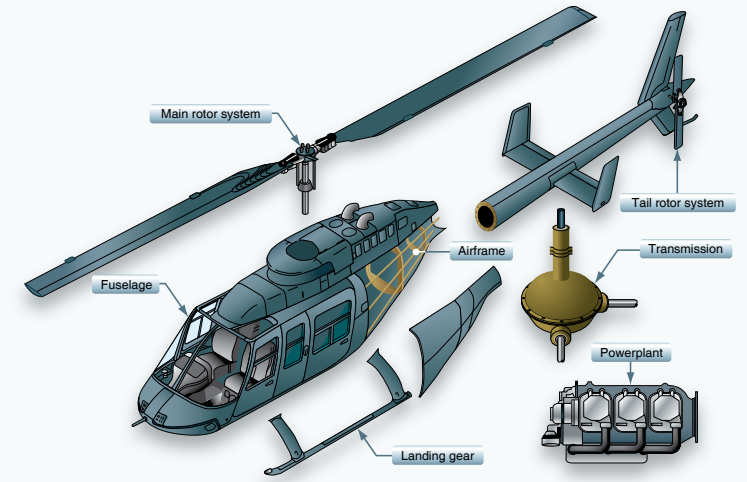
\includegraphics[width=0.8\linewidth]{gambar/komponenheli.png}
	\caption{Komponen helikopter secara umum \cite{handbook}.}
	\label{fig:komponenheli}
\end{figure}

\textit{Fuselage} badan helikopter merupakan bagian inti luar dari rangka yang menampung kabin berisi kru, penumpang, dan kargo. Kabin helikopter memiliki susunan tempat duduk yang berbeda-beda. Selain itu, badan helikopter juga berfungsi untuk memberikan ruang pada mesin, transmisi, avionik, kontrol penerbangan sumber power pada helikopter. Untuk sistem transmisi helikopter, mesin pada gigi rotor utama akan membuat poros rotor berputar. Ketika rotor berputar pada rpm mesin, kecepatan ujung rotor akan lebih cepat daripada kecepatan suara, kekuatan pada rotor harus ditingkatkan dan kelembaman dari giroskop akan menjadi sangat ekstrim. Terdapat bagian yang dinamakan \textit{clutch} (kopling) (gambar \ref{fig:clutch}) yaitu bagian yang terintegrasi dengan sistem transmisi. Bagian ini memungkinkan pilot untuk dapat mengatur kontak antara mesin dan poros penggerak \cite{wagtendonk2006principles}.

\begin{figure}[H]
	\begin{subfigure}{0.3\textwidth}
	\centering
	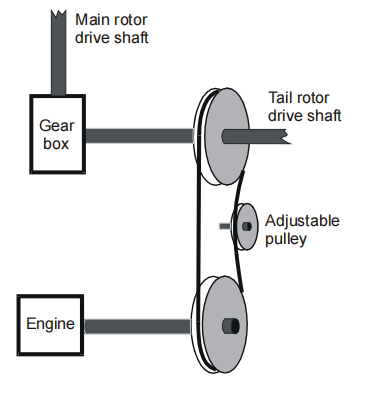
\includegraphics[width=\linewidth]{gambar/belt-driven_clutch.png}
	\caption{}
	\label{fig:belt-driven_clutch}
	\end{subfigure}
\centering
	\begin{subfigure}{0.3\textwidth}
	\centering
	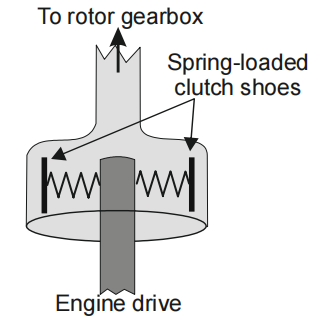
\includegraphics[width=\linewidth]{gambar/centrifugal_clutch.png}
	\caption{}
	\label{fig:centrifugal_clutch}
\end{subfigure}
	\caption{(a) Pengaturan kopling (\textit{clutch}) yang dihubungkan menggunakan sabuk. (b) Prinsip kopling sentrifugal \cite{handbook}.}
	\label{fig:clutch}
\end{figure}

Untuk mengatur pergerakannya, terdapat bagian komponen yang disebut dengan \textit{swashplate}, dapat dilihat pada gambar \ref{fig:swashplate}. Komponen ini dapat mengatur orientasi rotor utama dan jumlah gaya dorong rotor yang dihasilkan. Bearing (bola kecil) pada bagian \textit{swashplate} disesuaikan antara kedua piringan rotor yang bergerak. Sehingga gerakan piringan yang digerakkan oleh pilot akan berpindah ke rotor \cite{wagtendonk2006principles}.

\begin{figure}[H]
	\centering
	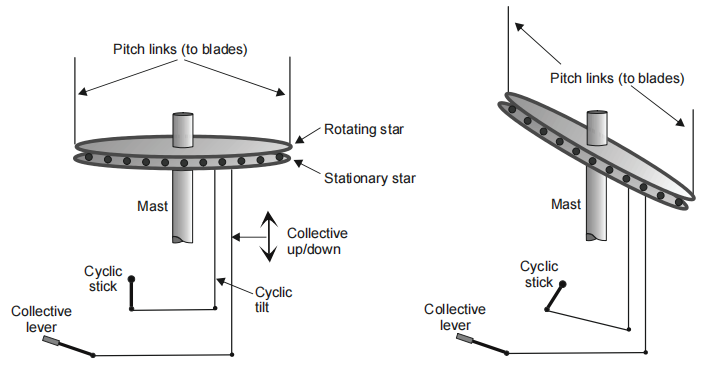
\includegraphics[width=0.7\linewidth]{gambar/swashplate.png}
	\caption{Mekanisme kontrol pada gerakan rotor utama \cite{handbook}.}
	\label{fig:swashplate}
\end{figure}
Sistem \textit{fully articulated rotor} mempunyai kemampuan pada rotornya untuk melakukan \textit{lead/lag} (gerakan kedepan dan belakang), \textit{flap} (gerakan atas dan bawah) dan \textit{feather} (berotasi pada sumbu radial) untuk merubah gaya angkat \cite{handbook} yang dapat dilihat pada gambar \ref{fig:fullyarticulated}.

\begin{figure}[H]
	\centering
	\begin{subfigure}{0.17\textwidth}
		\centering
		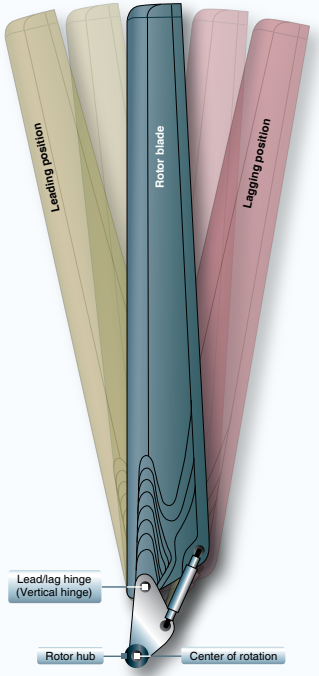
\includegraphics[width=\linewidth]{gambar/lead-lag.png}
		\caption{}
		\label{fig:lead/lag}
	\end{subfigure}
	\centering
	\begin{subfigure}{0.4\textwidth}
		\centering
		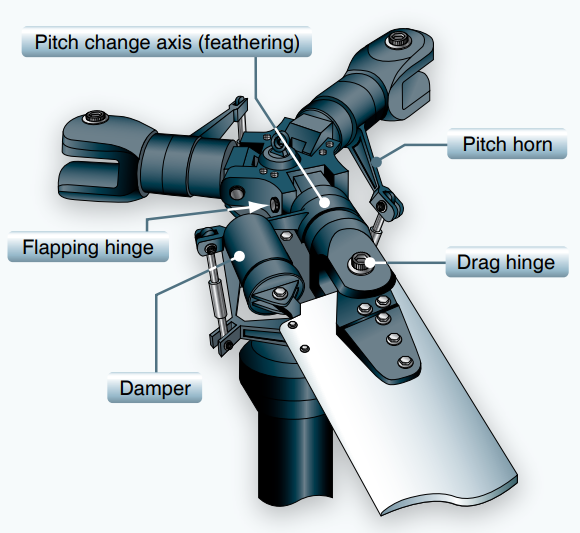
\includegraphics[width=\linewidth]{gambar/feather_flap.png}
		\caption{}
		\label{fig:featherflap}
	\end{subfigure}
	\caption{(a) Komponen \textit{lead/lag} membuat rotor dapat bergerak kedepan dan belakang pada bidangnya. (b) Komponen \textit{feather} dan \textit{flap} untuk gerakan rotasi pada arah radial serta bergerak atas bawah \cite{handbook}.}
	\label{fig:fullyarticulated}
\end{figure}

\begin{figure}[H]
	\centering
	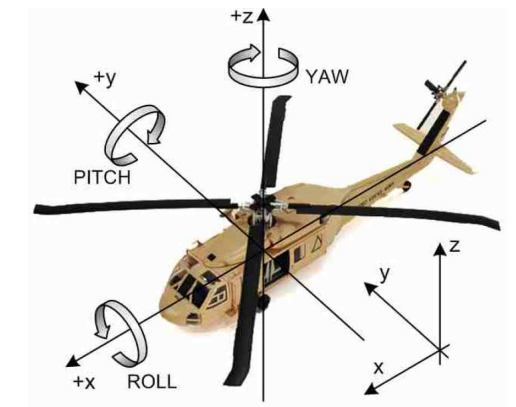
\includegraphics[width=0.68\linewidth]{gambar/roll-pitch-yaw.png}
	\caption{Orientasi arah helikopter \cite{Jhwang}.}
	\label{fig:orientasiheli}
\end{figure}

Saat rotor berputar, bilah pada rotor merespon \textit{input} dari kontrol untuk mengendalikan helikopter. Pusat daya angkat pada rotor akan bergerak karena respon yang diberikan \textit{input}, sehingga dapat menghasilkan gerakan \textit{pitch}, \textit{roll}, dan \textit{yaw} seperti yang dapat dilihat pada gambar \ref{fig:orientasiheli}. Arah gaya angkat ini bergantung pada \textit{input pitch} dan \textit{roll} dari pilot. Oleh karena itu, sudut \textit{feathering} pada setiap bilah akan berbanding lurus dengan gaya angkatnya, yaitu berubah saat berputar dengan rotor, gerakan ini disebut dengan \textit{cyclic control} \cite{handbook}.

Saat daya angkat meningkat, \textit{flapping hinge} akan mengayun ke arah atas tanpa kehilangan keseimbangan dengan gaya sentrifugal dari berat bilah rotor, dimana gaya tersebut akan tetap mempertahankan gerakannya untuk tetap pada bidang horizontal. Gaya sentrifugal pada dasarnya memiliki nilai yang konstan, namun gaya ayunan dipengaruhi oleh kecepatan naik, maju, dan berat helikopter. Sehingga saat bilah rotor berayun, pusat gravitasinya ikut berubah \cite{handbook}.

\section{\textit{Ground Resonance}}
\label{sec:groundresonance}

\textit{Ground resonance} adalah getaran dengan amplitudo besar yang disebabkan oleh osilasi pada helikopter yang sedang berada di tanah. Tanda awal resonansi ditandai dengan gerakan perlahan pada badan helikopter. Jika dibiarkan secara terus menerus, makana intensitas getaran akan semakin besar dan meningkat dengan cepat, sehingga berpotensi menyebabkan kerusakan pada pesawat \cite{wagtendonk2006principles}.

Fenomena \textit{ground resonance} merupakan getaran mekanis yang timbul secara otomatis dan terjadi pada sistem \textit{fully articulated rotor}. Engsel pada helikopter dengan sistem ini memberikan kebebasan pada masing-masing bilah rotor untuk bergerak dalam bidang rotasi rotor. Gerakan yang berlawanan dengan arah rotasi rotor disebut \textit{lagging}, sedangkan gerakan yang searah dengan rotasi disebut dengan \textit{leading}. Masing-masing bilah rotor memungkinkan untuk melakukan \textit{leading} atau \textit{lagging} untuk mengkompensasi perubahan drag yang terjadi ketika bilah rotor berayun karena adanya asimetri daya angkat dalam gerakan maju helikopter \cite{Eckert2007AnalyticalAA}.

Parameter yang penting terkait fenomena \textit{ground resonance} adalah frekuensi dan redaman pada mode \textit{lag} rotor, frekuensi dan redaman pada \textit{fuselage}, dan \textit{mode shape} pada \textit{fuselage}. Sehingga, identifikasi terhadap beban aerodinamik tidaklah menjadi penting. Karena dalam kondisi di ruang vakum pun \textit{ground resonance} juga tetap dapat terjadi pada helikopter \cite{bramwell2001bramwell}.

\begin{figure}[H]
	\centering
	\begin{subfigure}{0.4\textwidth}
		\centering
		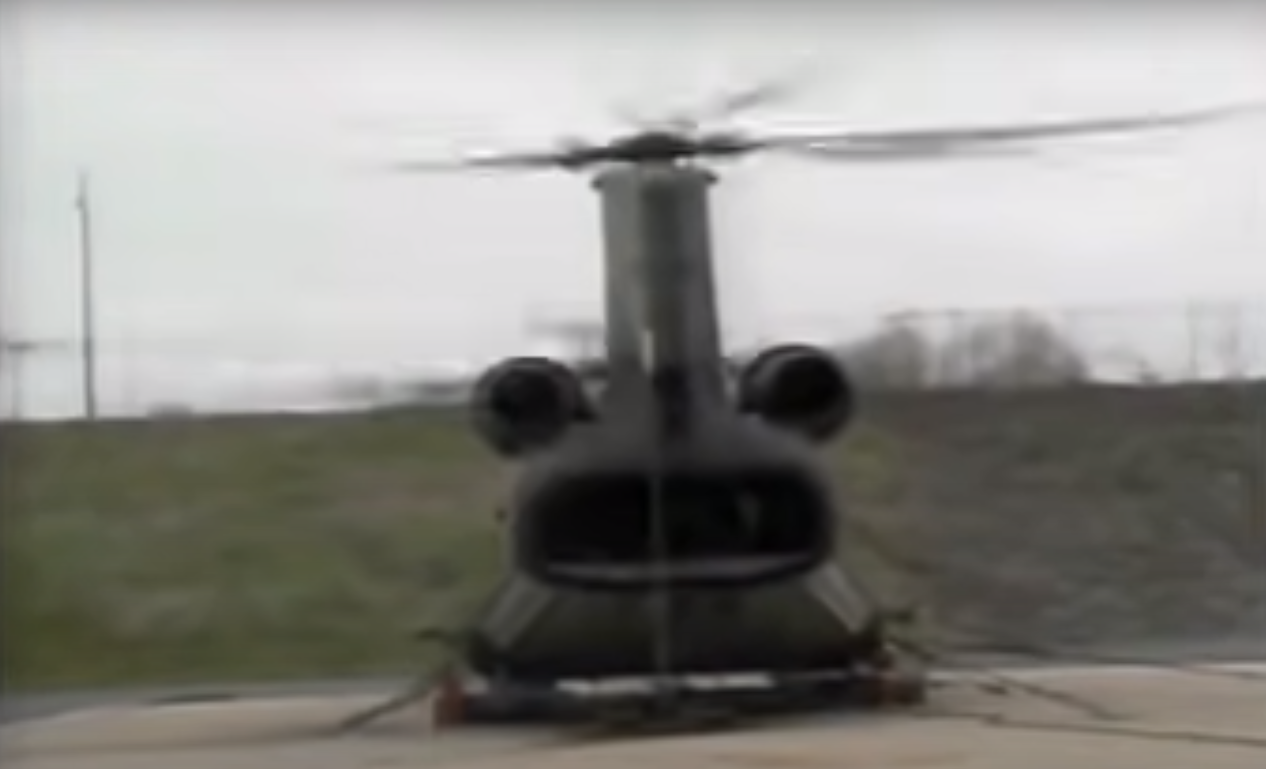
\includegraphics[width=\linewidth]{gambar/gr_1.png}
		\caption{}
		\label{fig:gr_1}
	\end{subfigure}
	\centering
	\begin{subfigure}{0.4\textwidth}
		\centering
		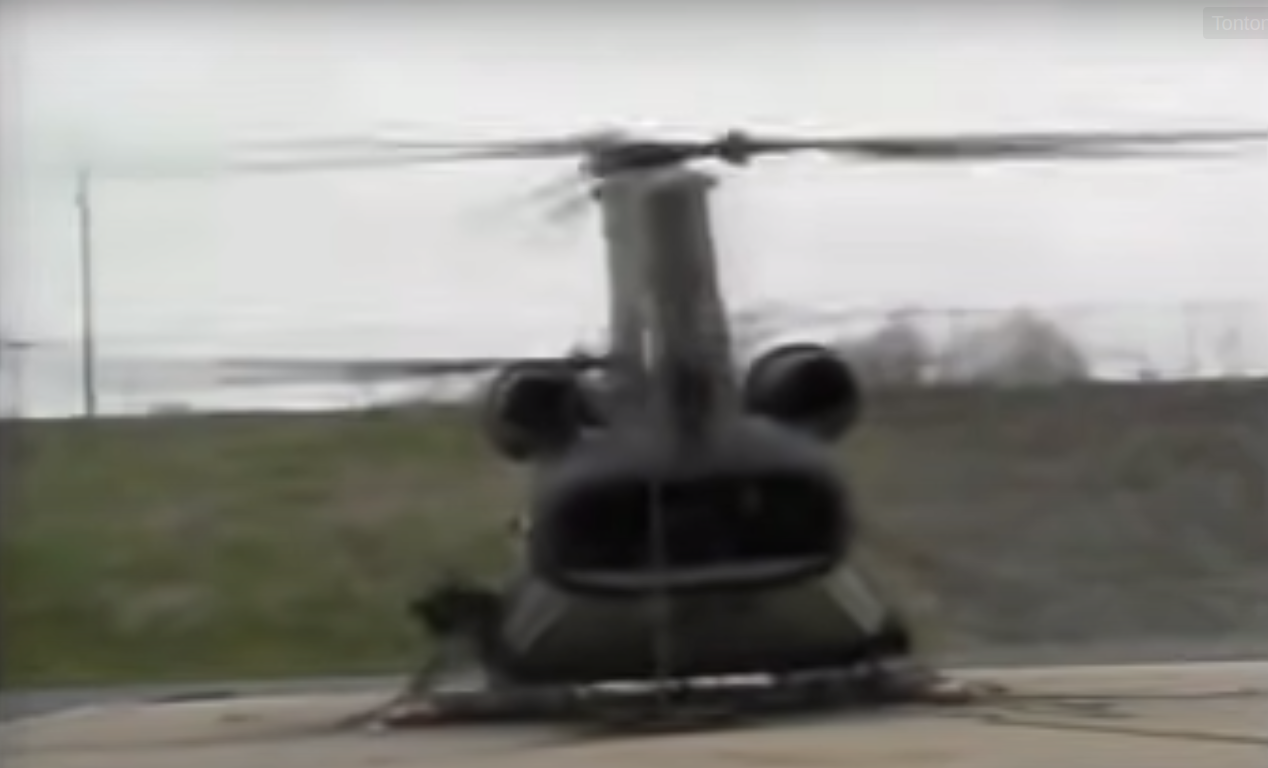
\includegraphics[width=\linewidth]{gambar/gr_2.png}
		\caption{}
		\label{fig:gr_2}
	\end{subfigure}
\\
	\centering
	\begin{subfigure}{0.4\textwidth}
		\centering
		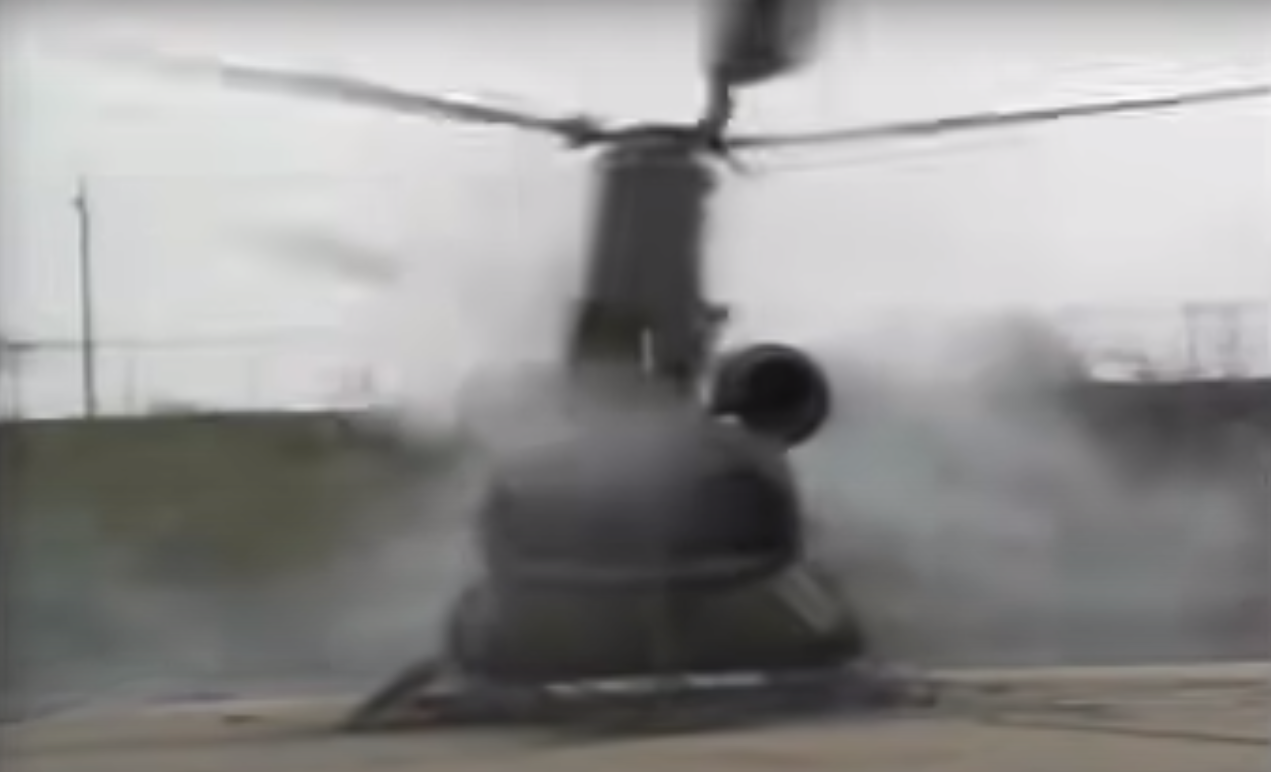
\includegraphics[width=\linewidth]{gambar/gr_3.png}
		\caption{}
		\label{fig:gr_3}
	\end{subfigure}
	\centering
	\begin{subfigure}{0.4\textwidth}
		\centering
		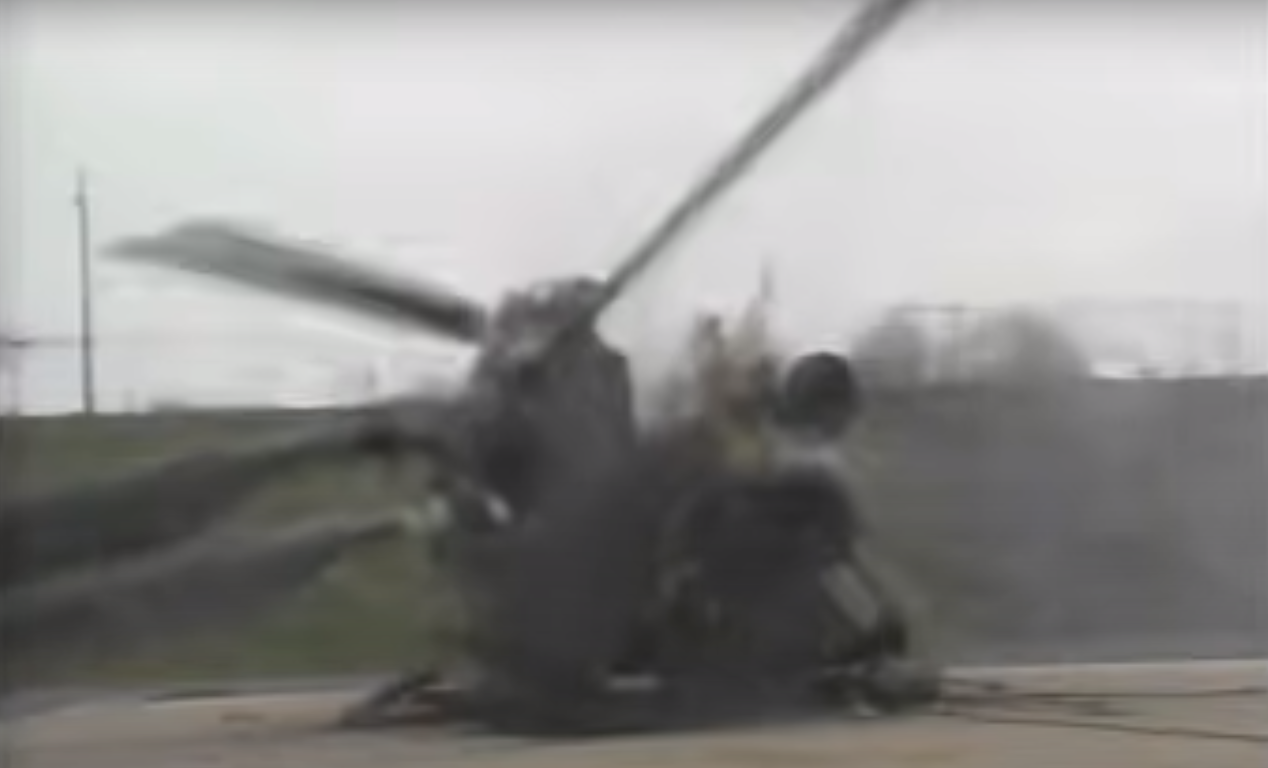
\includegraphics[width=\linewidth]{gambar/gr_4.png}
		\caption{}
		\label{fig:gr_4}
	\end{subfigure}
		\caption{(a) Kondisi saat helikopter stabil.(b) Sudah mulai terdapat getaran pada bagian kerangka helikopter (indikasi mulai terjadinya \textit{ground resonance}). (c) Terjadinya \textit{ground resonance} yang merusak bagian pada badan helikopter. (d) Pasca terjadinya \textit{ground resonance} pada helikopter.\\
		\urlstyle{rm}
		sumber: \url{https://www.youtube.com/watch?v=D2tHA7KmRME&t=3s}.}
		\label{fig:gr}
\end{figure}

Pada gambar \ref{fig:gr} menunjukkan situasi saat gerakan stabil \textit{lead/lag} tidak dapat mengkompensasi gerakan berlebih dalam bidang helikopter terhadap bilah rotor. Pusat gravitasi dari bilah rotor juga tidak lagi sejajar dengan penghubung pada rotor. Sehingga hal ini sangat berbahaya ketika helikopter bersentuhan dengan tanah. Posisi pusat gravitasi rotor yang tidak sejajar dengan penghubung rotor menghasilkan gaya sentrifugal yang tidak seimbang pada frekuensi tertentu \cite{Eckert2007AnalyticalAA}. Gaya tersebut menghasilkan gaya inersia periodik yang membuat seluruh badan helikopter bergetar terutama pada bagian pendaratannya ('\textit{chassis}' \textit{mode}). Jika salah satu frekuensi gaya inersia tersebut bertepatan dengan frekuensi pada '\textit{chassis}' \textit{mode} maka potensi terjadinya \textit{ground resonance} akan semakin besar \cite{bramwell2001bramwell}.

\begin{figure}[H]
	\centering
	\includegraphics[width=0.8\linewidth]{gambar/southwell_diagram.png}
	\caption{Diagram frekuensi \textit{chassis} dan rotor pada sistem \textit{fully articulated rotor} dengan sistem \textit{uncoupled}\cite{bramwell2001bramwell}.}
	\label{fig:southwell_diagram}
\end{figure}

Frekuensi yang dapat menyebabkan terjadinya fenomena \textit{ground resonance} dapat direpresentasikan dalam bentuk diagram seperti pada gambar \ref{fig:southwell_diagram}. Pada gambar tersebut, titik A merupakan frekuensi rotor saat \textit{hub} (penghubung) berada kondisi stasioner dan memiliki frekuensi yang lebih tinggi daripada frekuensi \textit{chassis mode} (garis putus-putus). 

Saat sistem \textit{uncoupled} mengacu pada kondisi saat gerakan pada rotor dan \textit{fuselage} dapat diperlakukan secara independen, tanpa ada pengaruh timbal balik yang signifikan. Sedangkan pada kondisi sebenarnya, helikopter memiliki sistem yang saling berhubungan satu sama lain, terutama antara sistem mekanik dan aerodinamik terhadap rotor dan \textit{fuselage}. Kondisi saling terhubung ini diakibatkan oleh perpindahan beban, getaran, dan energi antara kedua komponen tersebut. Ketika rotor menghasilkan gaya angkat atau berada pada kondisi \textit{idle}, maka hal tersebut akan menginduksi getaran dan gaya yang ditransimisikan ke badan helikopter \textit{fuselage}. 

Seiring dengan bertambahnya kecepatan pada rotor, frekuensi pada bilah rotor dan kecepatan pada rotor akan bertemu pada titik B dan C. Pada titik B, sistem masih dalam kondisi stabil. Sedangkan kondisi \textit{ground resonance} akan terjadi saat berada pada titik perpotongan di C. Pada kondisi sebenarnya (\textit{coupled}) memberikan visualisasi yang berbeda terhadap diagram pada gambar \ref{fig:southwell_diagram}. Saat kondisi ketidakstabilan terjadi, garis \textit{regressive mode} akan bertemu di sekitar titik C (gambar \ref{fig:southwell_coupled_diagram}), dan akan menyatu menjadi suatu rentang frekuensi yang mengindikasikan ketidakstabilan pada helikopter. 

\begin{figure}[H]
	\centering
	\includegraphics[width=0.75\linewidth]{gambar/southwell_coupled_diagram.png}
	\caption{Diagram frekuensi \textit{chassis} dan rotor pada sistem \textit{fully articulated rotor} dengan sistem \textit{coupled}\cite{bramwell2001bramwell}.}
	\label{fig:southwell_coupled_diagram}
\end{figure}


\section{Perhitungan Model Matematis}

Untuk dapat melakukan pendekatan secara analitik seperti yang telah diteliti oleh B.Bergeot et al \cite{BERGEOT201672}, diperlukan suatu model mekanik dari helikopter dengan derajat kebebasan minimum yang berpotensi mengalami fenomena \textit{ground resonance}. Oleh karena itu, dibutuhkan minimalnya sebanyak 5 derajat kebebasan (\textit{degree of freedom}/DOF). Helikopter terdiri atas \textit{fuselage} yang memiliki 4 bilah rotor dengan kecepatan konstan sebesar $\Omega$.

\begin{figure}[H]
	\centering 
	\begin{subfigure}{0.5\textwidth}
		\centering
		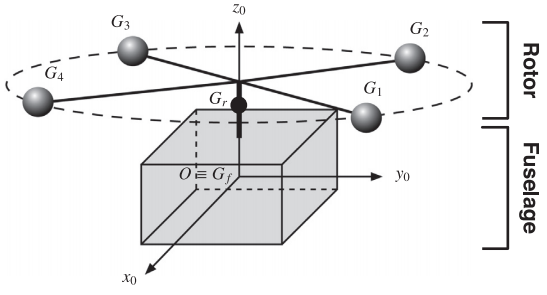
\includegraphics[width=\linewidth]{gambar/rotor_fuselage.png}
		\caption{}
		\label{fig:rotorfuselage}
	\end{subfigure}
	\centering
	\begin{subfigure}{0.35\textwidth}
		\centering
		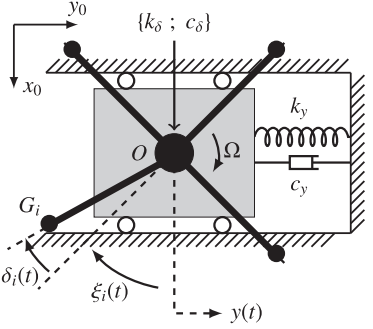
\includegraphics[width=\linewidth]{gambar/rotor_fuselage_topview.png}
		\caption{}
		\label{fig:topviewrotorfuslage}
	\end{subfigure}
	\caption{(a) Skema sederhana helikopter dengan 4 bilah rotor. (b) Skema helikopter dilihat dari atas \cite{BERGEOT201672}.}
	\label{fig:simplifiedmodel}
\end{figure}

Sistem koordinat kartesian digunakan dengan titik pusat di $O$. dengan $G_f$ merupakan pusat inersia \textit{fuselage} dan 3 sumbu kartesian pada sumbu-$x_0$, sumbu-$y_0$ dan sumbu-$z_0$ seperti yang terdapat pada gambar \ref{fig:rotorfuselage}. Kemudian terdapat $G_r$ yang merupakan pusat inersia rotor yang terletak di sumbu-$z_0$. Pada bagian \textit{fuselage} disederhanakan dengan representasi pemodelan yang tersusun seperti pada gambar \ref{fig:topviewrotorfuslage}, yaitu terdiri dari pegas, redaman dan massa dengan 1 arah translasi di sumbu-$y_0$. Selanjut pada arah translasi tersebut akan didefinisikan dalam domain waktu dengan koordinat $y(t)$. Pada masing-masing bilah rotor memiliki massa poin $G_i$ dengan [$i=1,2,3,4$], terletak pada jarak L dari sumbu-$z_0$. Sedangkan posisi pada bilah rotor ke-$i$ pada bidang-$x_0y_0$ sebagaimana persamaan \ref{eq:posisixy}.

\begin{equation}
\begin{cases}
x_{G_i} = L cos(\xi_i(t)+\delta_i(t))&(a) \\ 
y_{G_i} = y(t) + L sin(\xi_i(t)+\delta_i(t))&(b)
\end{cases}
\label{eq:posisixy}
\end{equation}

Dimana $\delta_i$ merupakan sudut \textit{lead/lag} pada bilah rotor ke-$i$. Sudut \textit{lead/lag} adalah perbedaan posisi bilah rotor saat waktu tertentu dengan posisi bilah rotor saat setimbangnya, yaitu $\xi_i(t)=\Omega t-(\pi/2)(i-1)$ sesuai pada gambar \ref{fig:topviewrotorfuslage}.

Persamaan gerak memiliki fungsi waktu untuk sistem 5 DOF pada helikopter, yaitu perpindahan \textit{fuselage} $y(t)$ dan 4 sudut \textit{lead/lag} $\delta_i(t)$. Kemudian pada tahap berikutnya adalah menurunkan persamaan gerak tersebut menggunakan metode Lagrange dengan variabel yang berkaitan ($T$=energi kinetik, $V$=energi potensial, dan $D$=disipasi energi Rayleigh) seperti pada persamaan \ref{eq:kinetik}, \ref{eq:potensial} dan \ref{eq:disipasi}.

\begin{align}
T &= \frac{1}{2}m_y\dot{y}^2 + \sum_{i=1}^{4}\frac{1}{2} m_{\delta} v^2_{\delta,i}
\label{eq:kinetik}
\\
V &= \frac{1}{2}k_yy^2+\sum_{i=1}^{4}\frac{1}{2}k_\delta \delta_i^2
\label{eq:potensial}
\\
D &= \frac{1}{2}c_y\dot{y}^2+\sum_{i=1}^{4}\frac{1}{2}c_\delta \dot{\delta}^2
\label{eq:disipasi}
\end{align}

Dengan bentuk umum persamaan dalam Lagrange seperti pada persamaan \ref{eq:lagrange_eq}.

\begin{align}
	\frac{d}{dt}\left(\frac{\partial T}{\partial \dot{q}_i}\right) - \frac{\partial T}{\partial q_i} + \frac{\partial D}{\partial \dot{q}_i} + \frac{\partial V}{\partial q_i} &= 0
	\label{eq:lagrange_eq}
\end{align}

Sehingga didapatkan:

\begin{equation}
	\begin{cases}
		(m_y+4m_\delta)\ddot{y}+c_y\dot{y}+k_yy+M_\delta\mathlarger{\sum}_{i=1}^{4}\left(\ddot{\delta_i}\cos(\xi_i+\delta_i)-(\Omega+\dot{\delta_i})^2\sin(\xi_i+\delta_i)\right) = 0 & (a) \\
		I_\delta\ddot{\delta_i}+c_\delta\dot{\delta_i}+k_\delta\delta_i+M_\delta \ddot{y}\cos(\xi_i+\delta_i)=0, \quad i=1,4 & (b)
	\end{cases}
	\label{eq:hasilmetodelagrang}
\end{equation}

Dengan ( $\dot{}$ ) merupakan tanda bahwa variabel tersebut telah diturunkan terhadap waktu $t$, $m_y$ merupakan massa \textit{fuselage}, $m_\delta$ adalah massa dari masing-masing bilah rotor. $M_\delta = m_\delta L$ dan $I_\delta = m_\delta L^2$ berturut-turut adalah momen statik dan momen inersia dari 1 bilah rotor. Subskrip $y$ adalah bagian dari \textit{fuselage} dan $\delta$ adalah bagian dari 1 buah bilah rotor. sehingga $c_y$ dan $c_\delta$ merupakan koefisien redaman dari \textit{fuselage} dan bilah rotor, $k_y$ dan $k_\delta$ adalah koefisien kekakuan linier dari \textit{fuselage} dan bilah rotor.

Untuk mendapatkan persamaan sistem yang \textit{time-invariant} (fungsi yang tidak bergantung mutlak pada waktu), maka persamaan \ref{eq:hasilmetodelagrang} harus dilinierisasi. Untuk itu, dilakukan asumsi bahwa sudut \textit{lead/lag} merupakan sudut yang sangat kecil ($\delta_i(t)<1$) kemudian menggunakan deret Taylor untuk mendapatkan sistem liniernya. Sehingga persamaan \ref{eq:hasilmetodelagrang} akan menjadi seperti persamaan \ref{eq:linearisasi_sudutkecil}.

\begin{equation}
	\begin{cases}
		(m_y+4m_\delta)\ddot{y}+c_y\dot{y}+k_yy+M_\delta\mathlarger{\sum}_{i=1}^{4}\left((\ddot{\delta}_i-\Omega^2\delta_i)\cos(\xi_i)-2\Omega \dot{\delta}_i\sin(\xi_i)\right) = 0 & (a) \\
		I_\delta\ddot{\delta}_i+c_\delta\dot{\delta}_i+k_\delta\delta_i+M_\delta \ddot{y}\cos(\xi_i)=0, \quad i=1,4 & (b)
	\end{cases}
\label{eq:linearisasi_sudutkecil}
\end{equation}

Transformasi Coleman melibatkan variabel yang mengubah gerakan masing-masing bilah rotor menjadi variabel gerakan kolektif. Untuk 4 bilah rotor akan terdapat 4 koordinat Coleman, diantaranya adalah $\delta_0$, $\delta_{1c}$, $\delta_{1s}$, dan $\delta_{cp}$ yang didefinisikan pada persamaan \ref{eq:colemantrans}.

\begin{equation}
\begin{aligned}
	\delta_0(t) &= \frac{1}{4}\mathlarger{\sum}_{i=1}^{4}\delta_i(t) && \text{(a)} \\
	\delta_{1c}(t) &= \frac{1}{2}\mathlarger{\sum}_{i=1}^{4}\delta_i(t) \cos(\xi_i(t)) && \text{(b)}\\
	\delta_{1s}(t) &= \frac{1}{2}\mathlarger{\sum}_{i=1}^{4}\delta_i(t) \sin(\xi_i(t)) && \text{(c)}\\
	\delta_{cp}(t) &= \frac{1}{4}\mathlarger{\sum}_{i=1}^{4}(-1)^i\delta_i(t) && \text{(d)}
\end{aligned}
\label{eq:colemantrans}
\end{equation}

Sebagaimana pada gambar \ref{fig:topviewrotorfuslage}, $\delta_i$ merupakan derajat kebebasan pada bilah rotor yang terlambat (\textit{lagging}), maka $\delta_0$ adalah \textit{lag} kolektif yang dimiliki rotor, sedangkan $\delta_{1c}$ dan $\delta_{1s}$ saling berhubungan dan merepresentasikan perpindahan dari pusat massa rotor $G_r$ pada bidangnya masing-masing di sumbu $x_0$ dan $y_0$ \cite{inproceedings}, sehingga didapatkan persamaan \ref{eq:pusatmassarotor}.

\begin{equation}
	\begin{cases}
		x_{G_r}(t) = -\mathlarger{\frac{L}{2}}\delta_{1s}(t)&(a) \\ 
		y_{G_r}(t) = \mathlarger{\frac{L}{2}}\delta_{1c}(t)&(b)
	\end{cases}
	\label{eq:pusatmassarotor}
\end{equation}

Dengan memasukkan variabel pada persamaan \ref{eq:colemantrans} ke persamaan \ref{eq:linearisasi_sudutkecil}, persamaan \ref{eq:linearisasi_sudutkecil}a dan \ref{eq:linearisasi_sudutkecil}b masing-masing akan persamaan \ref{eq:linearisasi}.

\begin{equation}
	\begin{cases}
	(m_y+4m_{\delta})\ddot{y}+c_y\dot{y}+k_yy+2M_{\delta}\ddot{\delta}_{1c}=0, &(a)\\
	I_{\delta}\ddot{\delta}_0+c_{\delta}\dot{\delta}_0+k_{\delta}\dot{\delta}_0=0&(b)\\
	I_{\delta}\ddot{\delta}_{1c}+c_{\delta}\dot{\delta}_{1c}+2I_{\delta}\Omega\dot{\delta}_{1s}+(k_{\delta}-I_{\delta}\Omega^2)\delta_{1c}+c_{\delta}\Omega\delta_{1s}+M_{\delta}\ddot{y}=0&(c)\\	I_{\delta}\ddot{\delta}_{1s}+c_{\delta}\dot{\delta}_{1s}-2I_{\delta}\Omega\dot{\delta}_{1c}+(k_{\delta}-I_{\delta}\Omega^2)\delta_{1s}-c_{\delta}\Omega\delta_{1c}=0&(d)\\
	I_{\delta}\ddot{\delta}_{cp}+c_{\delta}\dot{\delta}_{cp}+k_{\delta}\dot{\delta}_{cp}=0&(e)\\
	\end{cases}
	\label{eq:linearisasi}
\end{equation}

Pada persamaan \ref{eq:colemantrans} diatas, mode pada rotor hanya bergantung pada $\delta_{1c}$ dan $\delta_{1s}$, hal tersebut dikarenakan $\delta_{1c}$ dan $\delta_{1s}$ memengaruhi gaya dari rotor menuju ke \textit{fuselage}. Disisi lain, dari persamaan \ref{eq:linearisasi}, variabel $\delta_0$ dan $\delta_{cp}$ tidak saling berhubungan (\textit{uncoupled}) dan dapat diabaikan. Sehingga, hanya terdapat 3 derajat kebebasan dari pemodelan sederhana yang telah dilakukan diatas, yaitu $y$, $\delta_{1c}$, dan $\delta_{1s}$.

Persamaan gerak sederhana sesuai pada gambar \ref{fig:topviewrotorfuslage} dapat dituliskan dalam bentuk matriks pada persamaan \ref{eq:EOM}.

\begin{equation}
	\label{eq:EOM}
	\mathbf{M\ddot{X}}+(\mathbf{C}+\mathbf{G})\mathbf{\dot{X}}+\mathbf{KX}=\mathbf{0}
\end{equation}

Persamaan \ref{eq:linearisasi} dimuat dalam bentuk matriks dalam persamaan \ref{eq:EOM}. Dimana matriks $\mathbf{X}$, $\mathbf{M}$, $\mathbf{K}$, $\mathbf{C}$, dan $\mathbf{G}$ berturut-turut merupakan matriks derajat kebebasan, massa, kekakuan, redaman dan matriks giroskop dari sistem gerak. Masing-masing matriks tersebut didefinisikan pada persamaan \ref{eq:DOF} dan \ref{eq:matriks}.

\begin{equation}
	\label{eq:DOF}
	\mathbf{X}=[y \; \delta_{1c} \; \delta_{1s}]^t
\end{equation}

\begin{equation}
\begin{gathered}
	\mathbf{M}=\begin{bmatrix}
		1& \tilde{S}_d& 0\\
		\tilde{S}_c& 1& 0\\
		0& 0& 1
	\end{bmatrix}, \quad
	\mathbf{C}=\begin{bmatrix}
		\tilde{\lambda}_y& 0& 0\\
		0& \tilde{\lambda}_{\delta}& 0\\
		0& 0& \tilde{\lambda}_{\delta} 
	\end{bmatrix}, \\
	\mathbf{G}=\begin{bmatrix}
		0& 0& 0\\
		0& 0& 2\Omega\\
		0& -2\Omega& 0
	\end{bmatrix}, \
	\mathbf{K}=\begin{bmatrix}
		\omega^2_y& 0& 0\\
		0& \omega^2_{\delta}-\Omega^2& \tilde{\lambda}_{\delta}\Omega\\
		0& -\tilde{\lambda}_{\delta}\Omega& \omega^2_{\delta}-\Omega^2
	\end{bmatrix}
\end{gathered}
\label{eq:matriks}
\end{equation}

Dengan,

\begin{equation}
	\begin{gathered}
	\omega^2_y = \mathlarger{\frac{k_y}{(m_y+4m_{\delta})}},
	\quad 
	\omega^2_{\delta} = \mathlarger{\frac{k_{\delta}}{I_{\delta}}}, 
	\\
	\tilde{\lambda}_y = \mathlarger{\frac{c_y}{(m_y+4m_{\delta})}}, 
	\quad
	\tilde{\lambda}_{\delta} = \mathlarger{\frac{c_{\delta}}{I_{\delta}}}, 
	\\ 
	\tilde{S}_d = \mathlarger{\frac{2M_{\delta}}{(m_y+4m_{\delta})}}, 
	\quad 
	\tilde{S}_c = \mathlarger{\frac{M_{\delta}}{I_{\delta}}},
	\\
	I_{\delta} = m_{\delta}L^2, \quad M_{\delta}=m_{\delta}L
	\end{gathered}
\end{equation}

\textit{Ground resonance} berkaitan dengan analisis stabilitas pada persamaan \ref{eq:EOM}. Sehingga dapat didefinisikan dalam bentuk \textit{state-space}. Bentuk \textit{state-space} secara umum difenisikan pada persamaan \ref{eq:AdanQ}.

\begin{equation}
	\label{eq:AdanQ}
	\mathbf{\dot{Q}}=\mathbf{AQ}+\mathbf{BU}
\end{equation}

Dimana $\mathbf{\dot{Q}}$ adalah \textit{state vector} sebagai fungsi dari waktu, $\mathbf{A}$ dan $\mathbf{B}$ masing-masing adalah \textit{state matrix} dan \textit{input matrix} yang bernilai konstan. Sedangkan $\mathbf{U}$ adalah \textit{input} sebagai fungsi dari waktu. Karena pada persamaan \ref{eq:DOF} tidak memiliki \textit{input} maka persamaan dalam bentuk \textit{state-space} menjadi:

\begin{equation}
	\label{eq:state-space_simplified}
	\mathbf{\dot{Q}}=\mathbf{AQ}
\end{equation}

Dimana,

\begin{equation}
	\label{eq:state-space}
	\mathbf{Q}=[y \; \delta_{1c} \; \delta_{1s} \; \dot{y} \; \dot{\delta}_{1c} \; \dot{\delta}_{1s}]^t, \quad
	\mathbf{A}=\begin{bmatrix}
		\mathbf{0}& \mathbf{I}\\
		\mathbf{-M}^{-1}\mathbf{K}& \mathbf{-M}^{-1}(\mathbf{C}+\mathbf{G})
	\end{bmatrix}	
\end{equation}

Dengan $\mathbf{0}$ dan $\mathbf{I}$ masing-masing merupakan matriks bernilai $0$ dan matriks identitas berukuran 3x3. Solusi nilai eigen dan vektor eigen dari matriks $\mathbf{A}$ akan merepresentasikan fenomena dari \textit{ground resonance} melalui grafik imajiner terhadap kecepatan rotor $\Omega$ dan bagian riil terhadap kecepatan rotor $\Omega$.

\section{\textit{Logarithmic Decrement}}

Dalam suatu sistem periodik yang memiliki peredam. Pergerakan sistem tersebut seiring berjalannya waktu akan mengalami reduksi dan pada suatu waktu tertentu akan berhenti bergerak. Hal ini disebabkan oleh keberadaan peredam pada sistem. Penurunan amplitudo pada pergerakan suatu sistem yang teredam memiliki beberapa bentuk penurunan. Terdapat penurunan amplitudo yang terjadi secara linier dan logaritmik. Untuk penurunan yang bersifat logaritmik, terdapat peredam histeresis dan peredam viskositas. Pada bagian helikopter, peredam terdapat di bagian peredam hidrolik. Oleh karena itu, untuk analisis \textit{logarithmic decrement} pada helikopter digunakan peredam viskositas.

Dalam peredam viskositas, redaman terhadap penurunan amplitudo sistem terbagi menjadi 3 bentuk redaman, \textit{overdamped, critically damped,} dan \textit{underdamped}. Gambar \ref{fig:damping_motion} dan \ref{fig:underdamped} merupakan grafik yang menunjukkan gerakan penurunan amplitudo pada peredam viskositas. 

\begin{figure}[H]
	\centering
	\includegraphics[width=0.65\linewidth]{gambar/damping_motion.png}
	\caption{Gerakan pada sistem periodik pada peredam viskositas yang berbeda-beda \cite{rao2004mechanical}.}
	\label{fig:damping_motion}
\end{figure}

Penurunan secara logaritmik atau \textit{logarithmic decrement} merupakan paremeter spesifik yang dimiliki saat kondisi peredam viskositas berupa \textit{underdamped}. \textit{Logarithmic decrement} pada dasarnya juga merupakan parameter spesifik yang digunakan untuk menghitung koefisien redaman dari sistem liner \cite{Lojewski2020InfluenceOC}. 

\begin{figure}[H]
	\centering
	\includegraphics[width=0.7\linewidth]{gambar/underdamped.png}
	\caption{Grafik \textit{underdamped}.}
	\label{fig:underdamped}
\end{figure}

Persamaan \ref{eq:logdec} merupakan formulasi \textit{logarithmic decrement} pada kondisi \textit{underdamped}:

\begin{align}
	\delta = \frac{1}{m}ln\frac{x_1}{x_{m+1}}
	\label{eq:logdec}
\end{align}

Kemudian dari formulasi pada \ref{eq:logdec} dapat diformulasikan \textit{damping ratio} yang pada tahap berikutnya akan digunakan untuk pengolahan data pada helikopter.

\begin{align}
	\zeta=\frac{\delta}{\sqrt{\left( 2\pi \right)^2+\delta^2}}
\end{align}


\section{\textit{Finite Element Method}}

Metode elemen berhingga atau \textit{finite element method} merupakan sebuah metode numerik yang digunakan untuk mencari solusi dari mekanika kompleks serta permasalahan getaran dari suatu struktur. Pada metode ini, struktur asli pada objek dibagi menjadi elemen yang lebih kecil. Pada masing-masing elemen diasumsikan memiliki perilaku seperti bagian kontinu dari struktur yang disebut dengan elemen hingga (\textit{finite element}). Pada masing-masing elemen dihubungkan dengan suatu penghubung yang disebut dengan \textit{nodes} \cite{Lojewski2020InfluenceOC}.

Beberapa percobaan menggunakan analisis \textit{finite element} bertujuan untuk mendesain ulang dengan mengetahui terlebih dahulu deformasi yang terjadi pada suatu struktur, seperti yang dikejakan pada \cite{Gorecki2013}. Pada penelitian tersebut, dilakukan sebuah pemodelan pada helikopter menggunakan elemen stik model sebagai representasi bentuk simulasi pada pengujian resonansi sebenarnya dan langkah pertama untuk mengubah desain pada rotor helikopter. Gambar \ref{fig:ex_finite_element} merupakan contoh luaran yang didapatkan pada \cite{Gorecki2013}.

\begin{figure}[H]
	\centering
	\includegraphics[width=0.65\linewidth]{gambar/ex_finite_element.png}
	\caption{Salah satu contoh luaran pada \cite{Gorecki2013} untuk mencari deformasi dari simulasi pemodelan \textit{finite element}.}
	\label{fig:ex_finite_element}
\end{figure}

Pada gambar \ref{fig:ex_finite_element} merupakan salah satu contoh analisis menggunakan elemen hingga. Secara matematis, deformasi atau perpindahan secara transversal pada suatu elemen tertentu dapat diekspresikan dalam persamaan \ref{eq:FEM}.

\begin{align}
	\label{eq:FEM}
	w(x,y,t)=\sum_{i=1}^{n}N_i(x,y)w_i(t)
\end{align}

$N_i(x,y)$ merupakan \textit{shape function} yang berkorelasi dengan perpindahan pada \textit{nodes} $w_i(t)$ dan n merupakan penghubung ke-n. Jika diberikan gaya dari luar sebesar $f(x,y,t)$ pada elemennya. Maka gaya tersebut memiliki ekivalensi dengan bentuk $f_i(t)(i=1, 2, ...., n)$. Kemudian dapat didefinisikan dari energi kinetik serta potensial dari masing-masing elemen dalam bentuk matriks vektor ${\overrightarrow{\textbf{W}}}$. 

\begin{align}
	T=\frac{1}{2}\dot{\overrightarrow{\textbf{W}^T}}[m]\dot{\overrightarrow{\textbf{W}}}
	\label{eq:kinetik_FEM}
\end{align}

\begin{align}
	V=\frac{1}{2}\overrightarrow{\textbf{W}^T}[k]\overrightarrow{\textbf{W}}
	\label{eq:potensial_FEM}
\end{align}

dengan,

\begin{align*}
\overrightarrow{\textbf{W}}=\left\{ \begin{matrix} w_1(t) \\ w_2(t) \\ w_3(t) \\ .\\ .\\ .\\ w_n(t) \end{matrix}\right\}, \dot{\overrightarrow{\textbf{W}}}=\left\{ \begin{matrix} \dot{w}_1(t) \\ \dot{w}_2(t) \\ \dot{w}_3(t) \\ .\\ .\\ .\\ \dot{w}_n(t) \end{matrix}\right\}=\left\{ \begin{matrix} dw_1/dt \\ dw_2/dt \\ dw_3/dt \\ .\\ .\\ .\\ dw_n/dt \end{matrix}\right\}
\end{align*}

Dimana [m] dan [k] merupakan matriks massa dan kekakuan dari elemen. Apabila pada persamaan \ref{eq:kinetik_FEM} dan \ref{eq:potensial_FEM} disubtitusikan dengan menggunakan persamaan Lagrange \ref{eq:lagrange_eq}. Maka persamaan tersebut akan menjadi:

\begin{align}
	[m]\ddot{\overrightarrow{\textbf{W}}}+[k]\overrightarrow{\textbf{W}}=\overrightarrow{f}
	\label{eq:kinetik+potensial_lagrange}
\end{align}

$\overrightarrow{f}$ merupakan vektor gaya pada penghubung dan $\ddot{\overrightarrow{\textbf{W}}}$ merupakan percepatan pada \textit{nodes}. Dengan $\ddot{\overrightarrow{\textbf{W}}}$ merupakan turunan dari $\dot{\overrightarrow{\textbf{W}}}$ \cite{rao2004mechanical}. Semua proses matematis ini akan diproses menggunakan komputasi yang dimiliki oleh \textit{software} FEMAP dalam mencari penyelesaian serta memberikan representasi gerakan \textit{mode shape} pada helikopter yang akan dimodelkan.

\section{\textit{Ground Vibration Test} (GVT)}
\label{sec:GVT}

\begin{figure}[H]
	\centering
	\includegraphics[width=0.6\linewidth]{gambar/Eksiter_landing.png}
	\caption{Sumber penggetar pada bagian pendaratan \textit{aircraft} \cite{lubrina:hal-01059708}.}
	\label{fig:shaker_landing}
\end{figure}

\begin{figure}[H]
	\centering
	\includegraphics[width=0.6\linewidth]{gambar/Shaker_mainrotor.png}
	\caption{Penempatan \textit{shaker} pada bagian rotor utama \cite{Ciavarella2018AnEH}.}
	\label{fig:shaker_rotor}
\end{figure}

\textit{Ground Vibration Test} (GVT) memiliki tujuan utama untuk memberikan informasi mengenai karakterisasi struktur objek \textit{aircraft}. Dengan GVT dapat dilakukan identifikasi terhadap parameter modal eksperimental seperti frekuensi eigen, mode eigen, rasio redaman, massa umum, dan fungsi transfer yang menggambarkan perilaku dinamis struktural dari \textit{aircraft} yang diuji. Selain didapatkannya informasi tentang dinamika struktural \textit{aircraft}, juga akan didapatkan informasi fundamental untuk memvalidasi serta model terbaru dari \textit{Finite Element} (FE) dinamis \cite{Ciavarella2018AnEH}.

Untuk mendapatkan kualitas pengujian data yang baik, diperlukan pemahaman tentang struktur \textit{rotorcraft} serta persiapan yang tepat dalam melakukan GVT \cite{Ciavarella2018AnEH}. Selain itu, diperlukan juga peralatan yang memadai untuk memberikan \textit{input} getaran dalam mengukur respon getaran. Dengan ukuran dan berat yang cukup besar, rentang frekuensi yang dianalisis umum berada pada frekuensi rendah. Berdasarkan apa yang telah dikerjakan pada \cite{lubrina:hal-01059708} (contoh peletakan ada pada gambar \ref{fig:shaker_landing}) dilakukan analisis pada rentang frekuensi yang tidak lebih tinggi dari 50Hz. Batas frekuensi rendah dari rentang frekuensi bergantung pada karakteristik suspensi. Sedangkan pengukuran untuk melakukan identifikasi frekuensi eigen pada \textit{rigid body} batas frekuensi terendahnya tidak lebih kecil dari 1Hz. Sehingga sumber penggetar (\textit{shaker}) harus memiliki eksitasi hetaran pada frekuensi eigen yang rendah dengan kekuatan yang cukup \cite{lubrina:hal-01059708}. Disisi lain pada penelitian \cite{Ciavarella2018AnEH} memberikan 4 \textit{shaker} pada bagian rotor utama helikopter dengan arah lateral dan vertikal yang berkisar pada rentang 220 hingga 2200N (gambar \ref{fig:shaker_rotor}).

Untuk tujuan mitigasi, dilakukan 2 pengukuran gaya eksitasi dengan prinsip pengukuran yang berbeda. Pertama, gaya eksitasi diukur menggunakan alat ukur piezo elektrik. Kedua, gaya eksitasi diukur menggunakan arus koil yang disediakan oleh \textit{power amplifier} pada \textit{shaker}. Sensor perpindahan digunakan untuk mengukur perpindahan relatif dari armatur \textit{shaker} pada tempat peletakan \textit{shaker}. Sedangkan untuk mengukur respon vibrasi secara utama menggunakan akselerometer dalam pengukurannya. Pada penelitian \cite{lubrina:hal-01059708} digunakan sebanyak 500 sensor akselerometer untuk melakukan GVT, kemudian data hasil sensor diakuisisi menggunakan \textit{multichannel dynamic data} dari LMS Scadas III unutk selanjutnya diatur dengan perangkat lunak seperti Test.Lab \textit{software}.


\section{AS 565 MBe Panther}
\label{sec:AS565MBe}

\begin{figure}[H]
	\centering
	\includegraphics[width=0.6\linewidth]{gambar/AS565pic.png}
	\caption{Potret AS 565 MBe Panther saat mengudara.}
	\label{fig:AS565pic}
\end{figure}

AS 565 MBe Panther seperti pada gambar \ref{fig:AS565pic} adalah versi militer dari Eurocopter AS 365 Dauphin helikopter dengan mesin ganda dan bobot menengah yang multiguna. Helikopter ini dapat digunakan untuk berbagai peran militer, termasuk serangan tempur, dukungan tembakan, perang anti-kapal selam, perang anti-permukaan, pencarian dan penyelamatan, dan evakuasi medis \cite{AS565MBe}. Helikopter AS 565 MBe Panther dapat dimodifikasi sedemikian rupa untuk selanjutnya ditambahkan fitur persenjataan yang dapat mendukung kinerja helikopter ini dalam melakukan tugasnya. \textit{Profile} mengenai helikopter AS 565 MBe Panther dapat dilihat pada gambar \ref{fig:AS565MBe}. Dari informasi tersebut, helikopter ini memiliki berat maksimum agar helikopter dapat terbang adalah sebesar 4500kg. Sehingga, apabila modifikasi yang dilakukan pada helikopter merupakan modifikasi penambahan massa tanpa adanya modifikasi pada rotor, maka massa 4500kg akan menjadi batas maksimum modifikasi tersebut. Adapun potret dan dimensi spesifik terkait helikopter AS 565 MBe Panther dapat dilihat pada gambar \ref{fig:AS565MBe}, \ref{fig:as565mbe_atas}, \ref{fig:as565mbe_depan} dan \ref{fig:as565mbe_samping}.

\begin{figure}[H]
	\centering
	\includegraphics[width=0.7\linewidth]{gambar/Propertis_AS565MBe.png}
	\caption{\textit{Profile} helikopter AS 565 MBe Panther.}
	\label{fig:AS565MBe}
\end{figure}

\begin{figure}[H]
	\centering
	\includegraphics[width=0.9\linewidth]{gambar/as565_samping.png}
	\caption{Dimensi Helikopter AS 565 MBe Panther tampak samping.}
	\label{fig:as565mbe_samping}
\end{figure}

\begin{figure}[H]
	\centering
	\includegraphics[width=0.9\linewidth]{gambar/as565_atas.png}
	\caption{Dimensi Helikopter AS 565 MBe Panther tampak atas.}
	\label{fig:as565mbe_atas}
\end{figure}

\begin{figure}[H]
	\centering
	\includegraphics[width=0.7\linewidth]{gambar/as565_depan.png}
	\caption{Dimensi Helikopter AS 565 MBe Panther tampak depan.}
	\label{fig:as565mbe_depan}
\end{figure}
\cleardoublepage

% Bab 3 desain dan implementasi
\chapter{METODOLOGI PENELITIAN}
\label{chap:metodologipenelitian}

% Ubah bagian-bagian berikut dengan isi dari desain dan implementasi

Untuk mencapai tujuan dalam tugas akhir ini, dilakukan beberapa tahap yang dimulai dengan memahami fenomena \textit{ground resonance} pada helikopter melalui studi pustaka serta teori pendukung. Berikutnya adalah melakukan perumusan terhadap permasalahan yang akan diselesaikan, dalam hal ini adalah terkait dengan fenomena \textit{ground resonance} helikopter modifikasi PTDI.

Terdapat 3 pekerjaan yang dikerjaan secara paralel dan berurutan, yaitu pengukuran di tanah \textit{ground test} helikopter, perhitungan matematis secara teori dan komputasi Matlab serta simulasi menggunakan \textit{software} Femap. Sehingga bila direpresentasikan dalam bentuk alur pengerjaannya dapat dilihat pada gambar \ref{fig:TA_flow-Page-1.jpg} dan \ref{fig:TA_flow-Page-2.jpg}.
 
\begin{figure}[H]
	\centering
	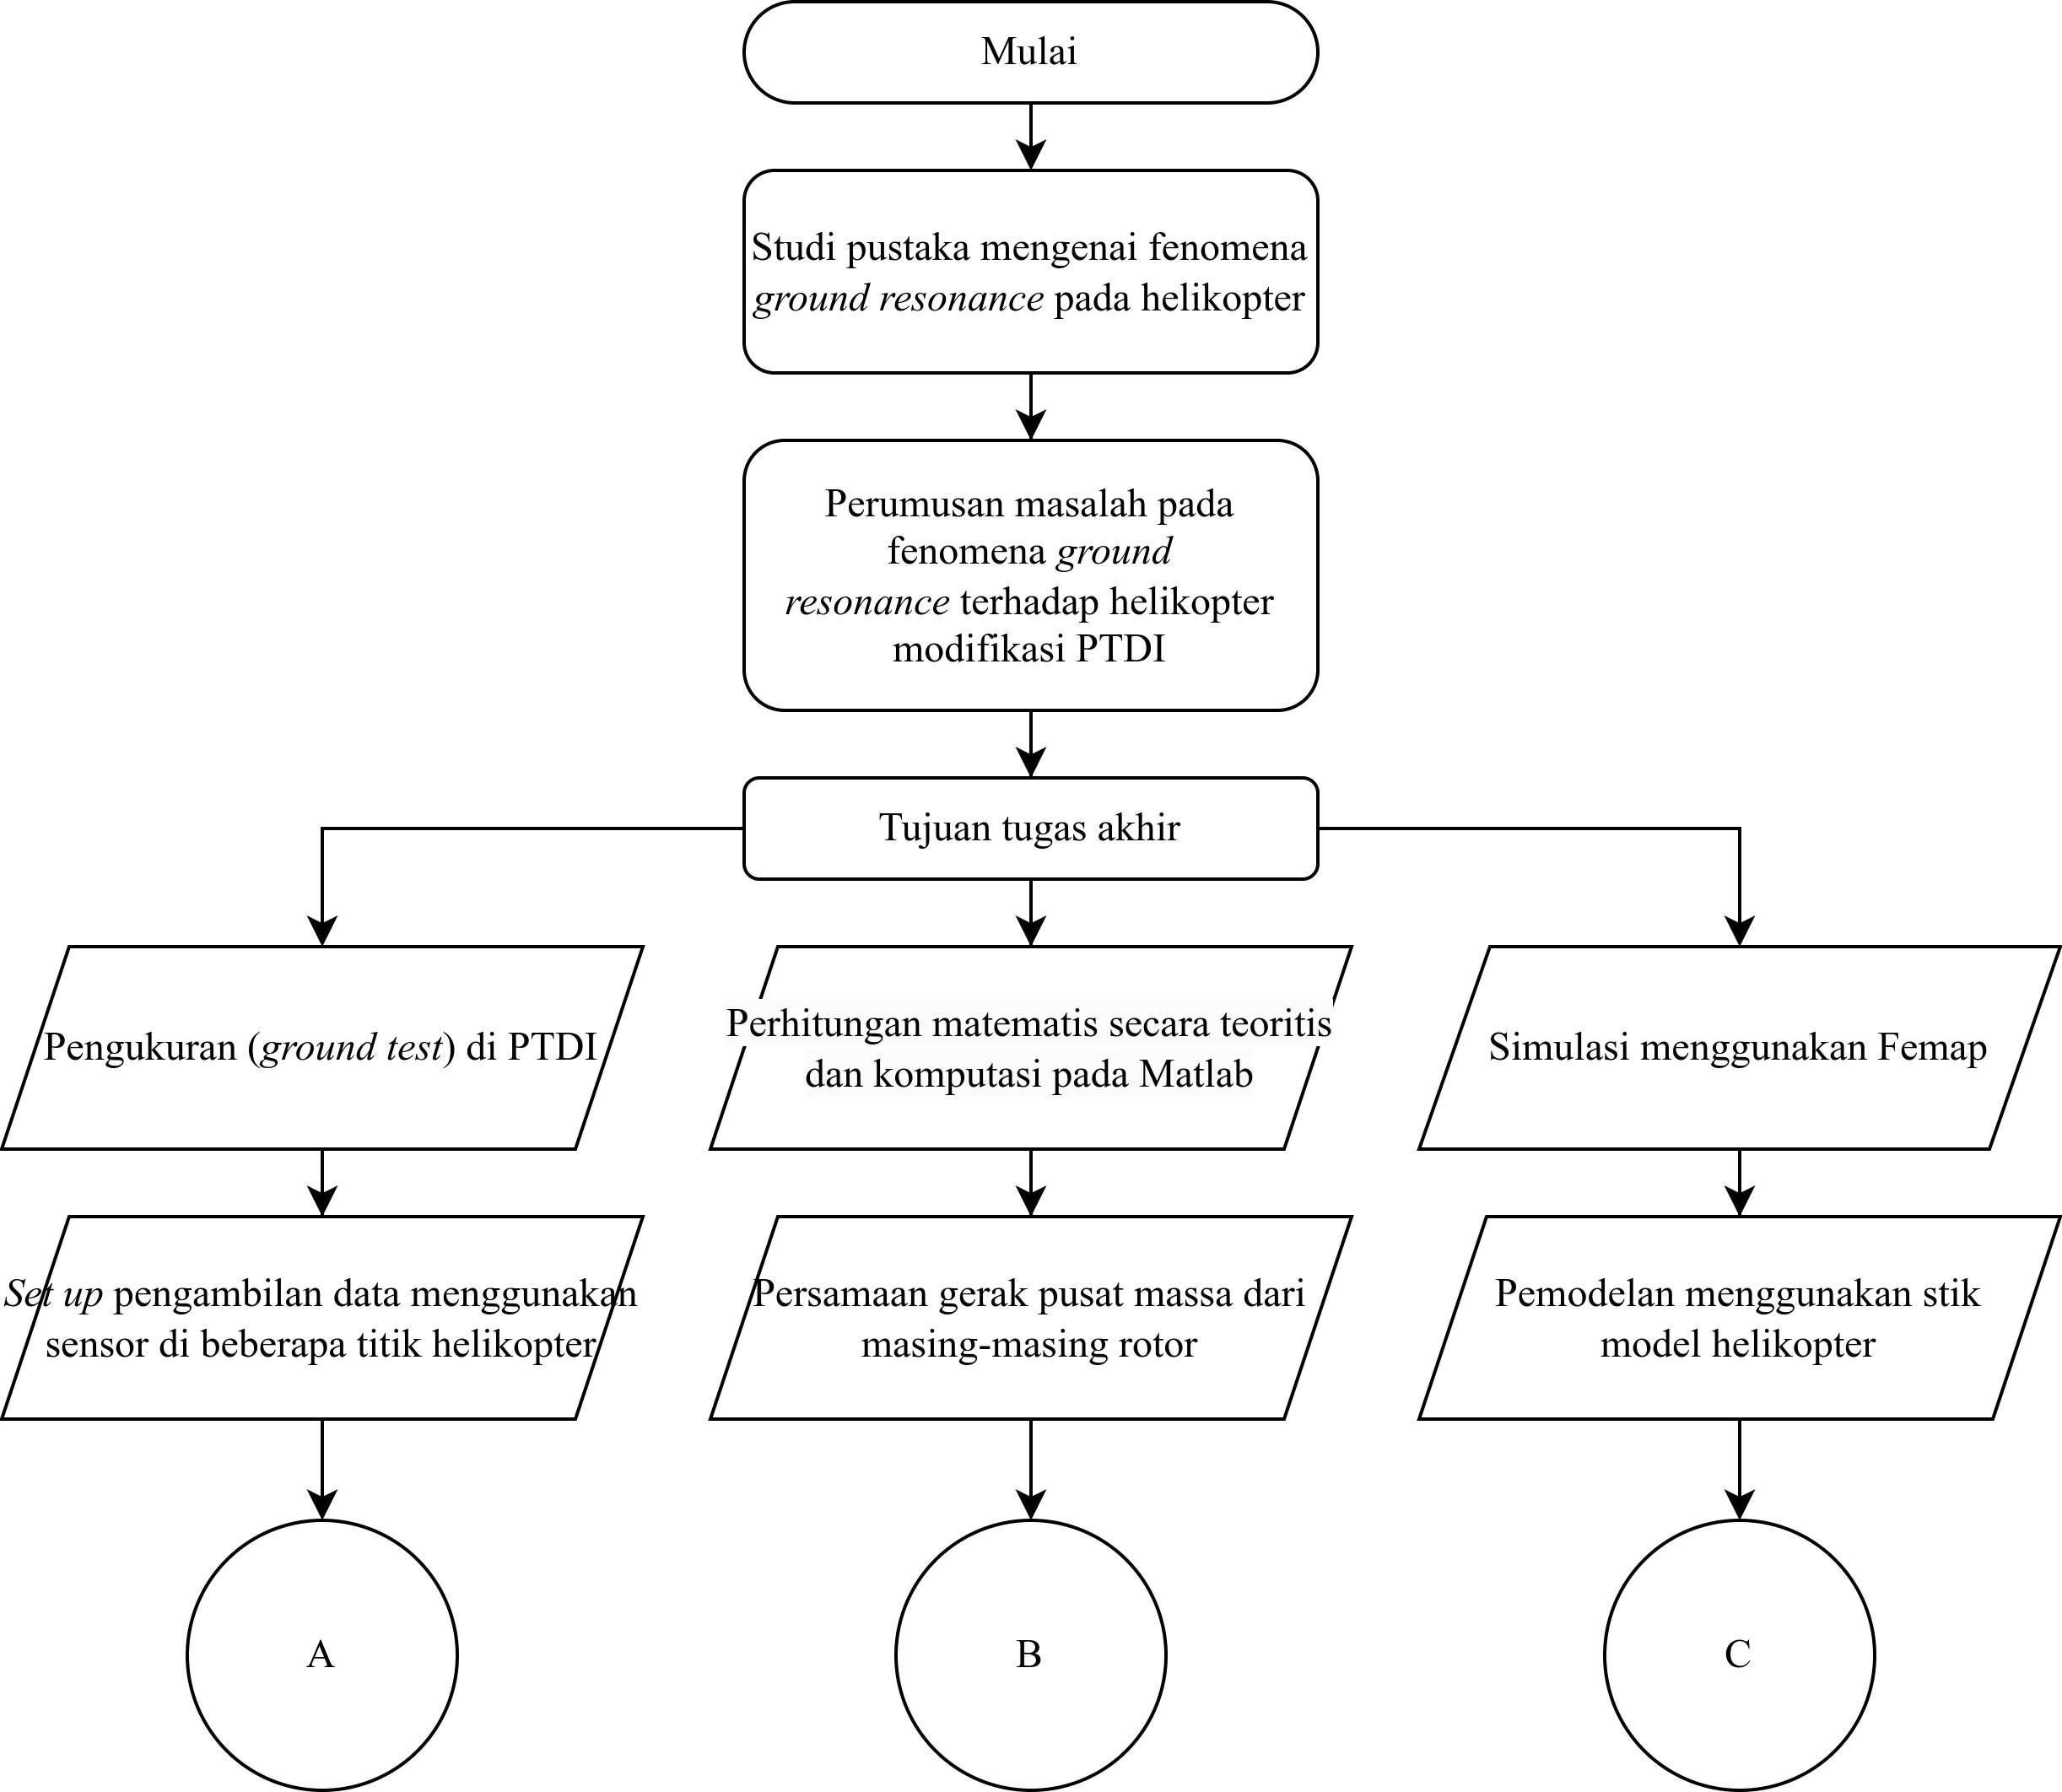
\includegraphics[width=1\linewidth]{gambar/TA_flow-Page-1.jpg}
	\caption{Diagram alir pengerjaan Tugas Akhir bagian 1.}
	\label{fig:TA_flow-Page-1.jpg}
\end{figure}

\begin{figure}[H]
	\centering
	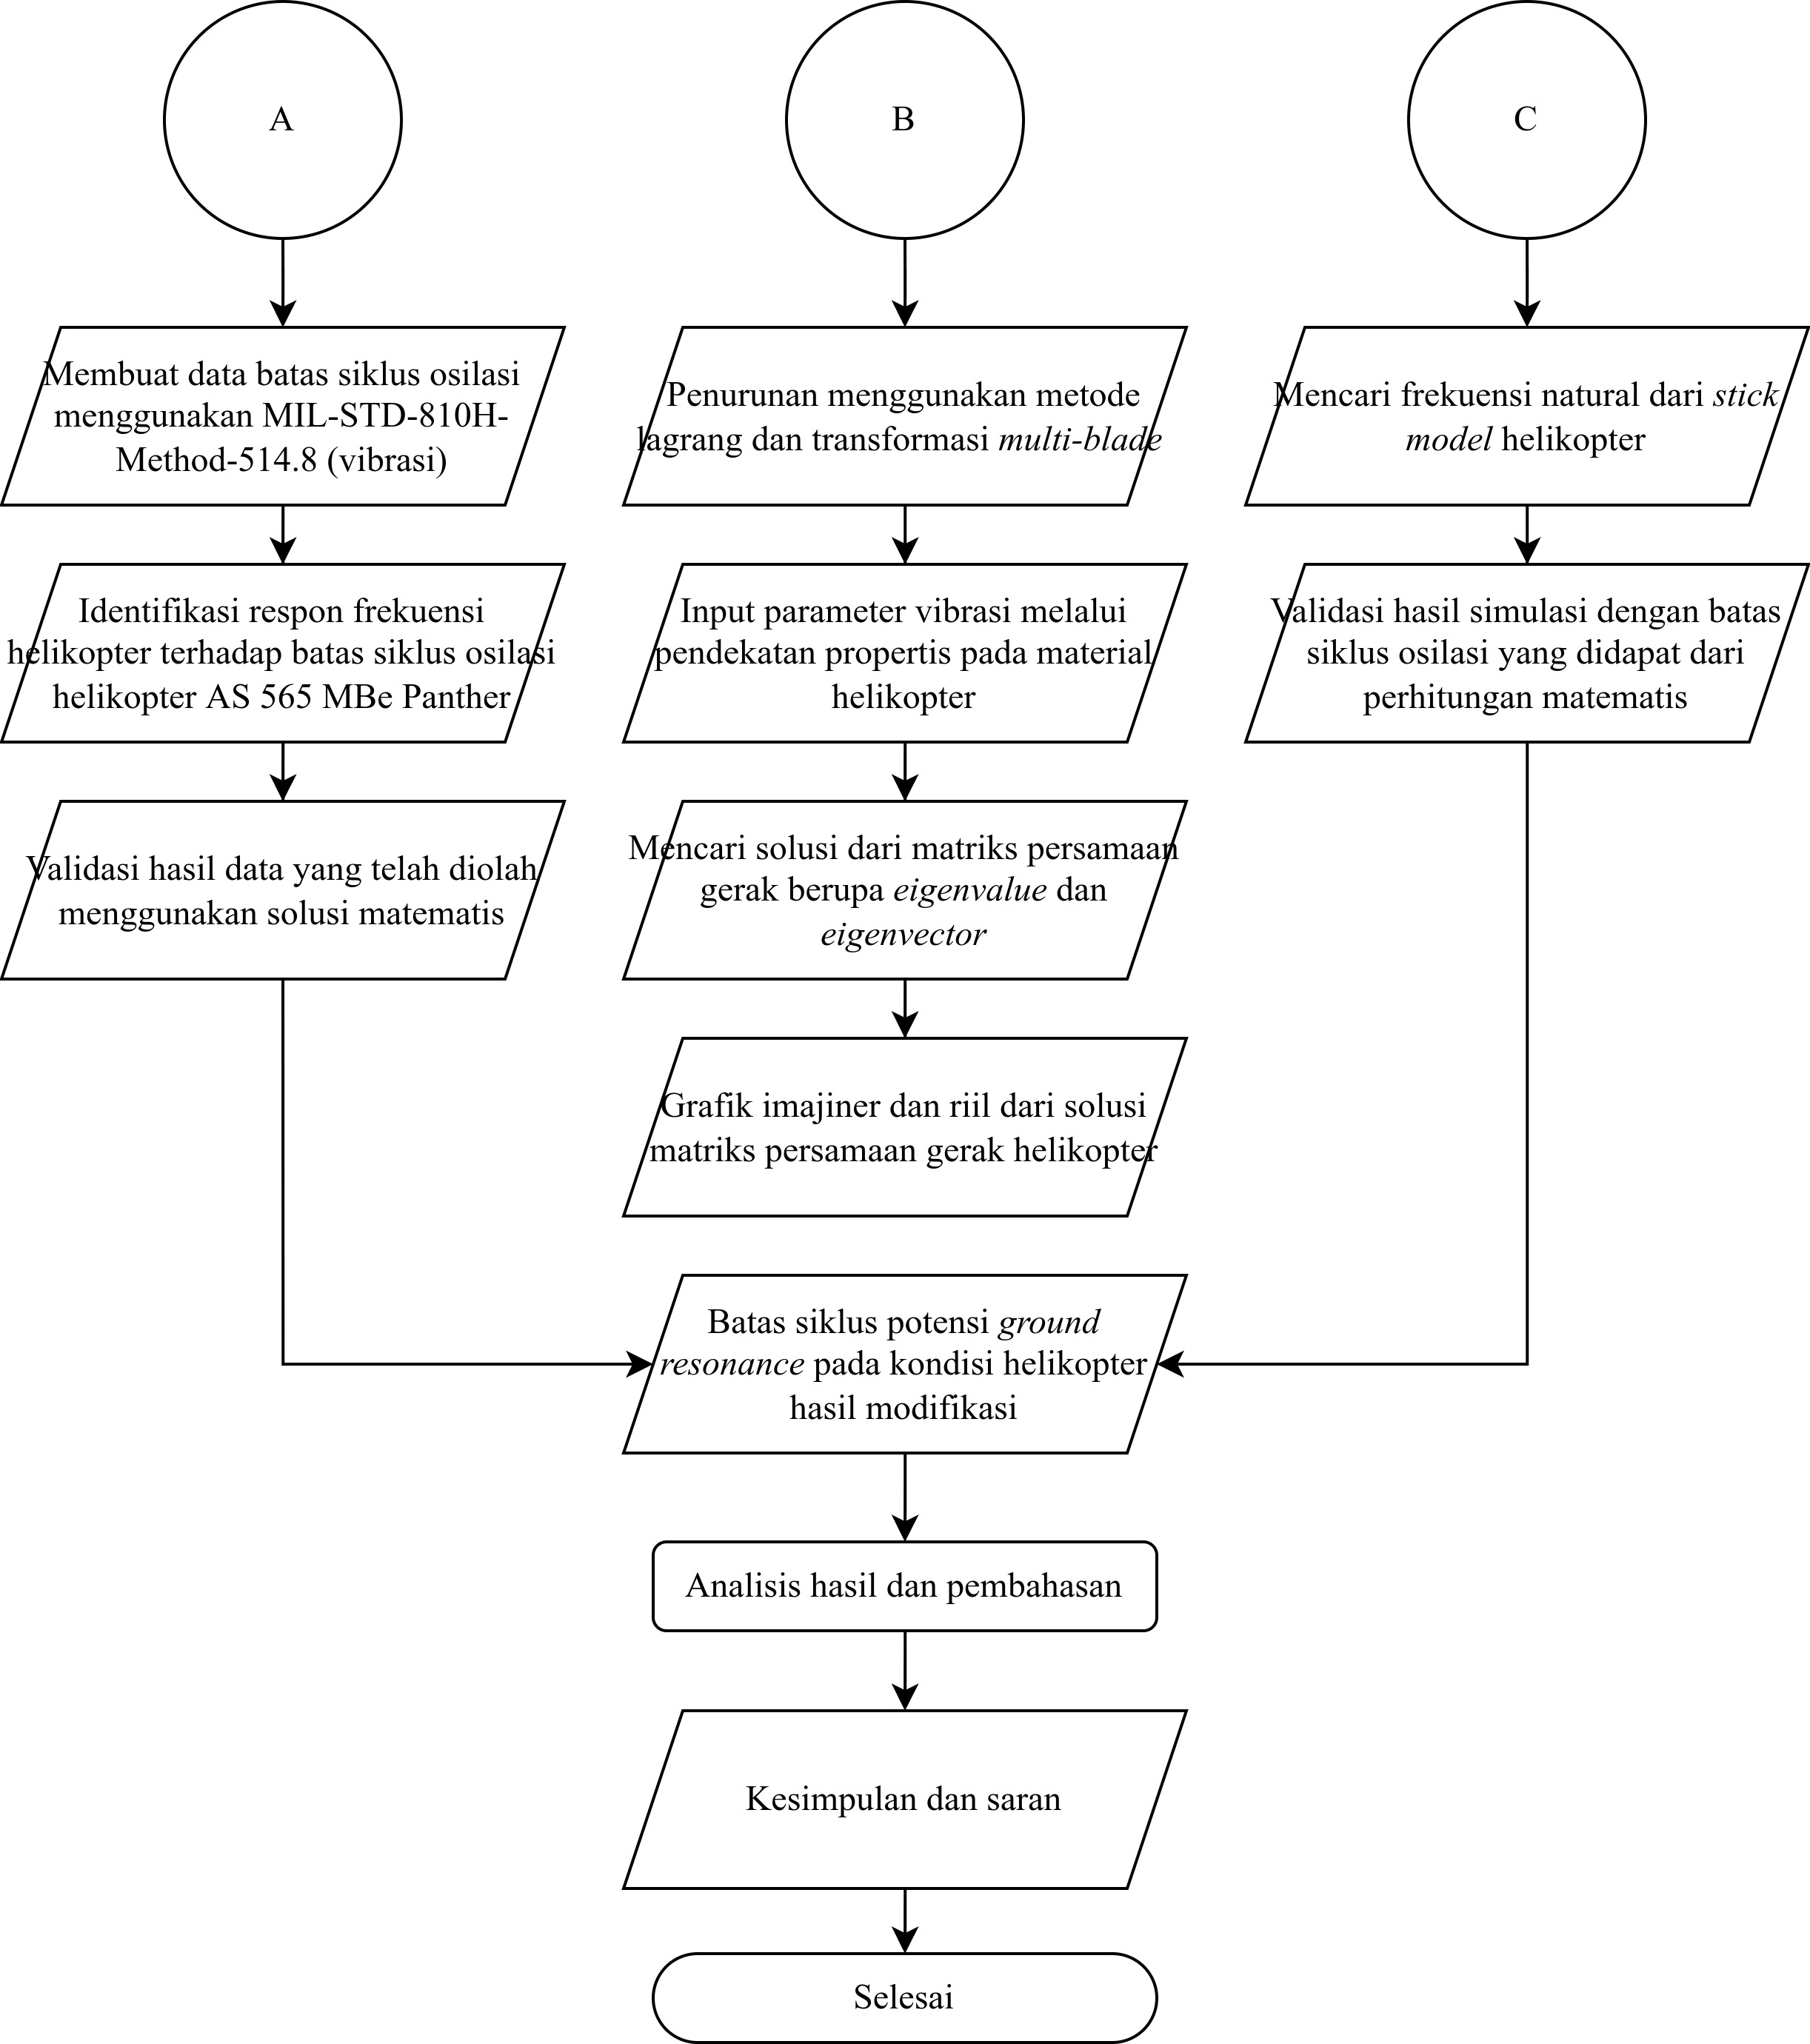
\includegraphics[width=0.95\linewidth]{gambar/TA_flow-Page-2.jpg}
	\caption{Diagram alir pengerjaan Tugas Akhir bagian 2.}
	\label{fig:TA_flow-Page-2.jpg}
\end{figure}

\section{Studi Pustaka}
\label{sec:studipustaka}

Studi pustaka merupakan tahap untuk membaca dan memahami referensi solusi serta metode peneliti sebelumnya berkaitan dengan \textit{ground resonance} pada helikopter. Beberapa referensi yang mendukung terhadap topik ini adalah mengenai metode pengolahan data hasil pengukuran menggunakan MIL-STD-810H-Method-514.8 (vibrasi), perhitungan matematis yang menggunakan konsep dasar dari parameter pegas-peredam-massa, penyelesaian matematis dengan menggunakan lagrang, transformasi \textit{multiblade} matriks, dan solusi eigen dengan bantuan komputasi Matlab. Kemudian referensi lain berupa informasi untuk pemakaian \textit{software} Femap dalam aspek simulasinya.

\section{Pengambilan Data \textit{Ground Test}}
  \label{sec:pengukurandata}

Pengambilan data \textit{ground test} dilakukan dengan mengikuti mekanisme yang telah ditetapkan oleh PTDI. Terdapat 2 pengukuran yang dilakukan, pertama adalah pengukuran terhadap \textit{damping ratio} dari respon helikopter terhadap impuls yang diberikan oleh pilot. Kedua, adalah pengukuran yang didapatkan menggunakan sensor akselerometer yang dipasangkan di beberapa titik pada helikopter.

\subsection{Pengukuran Data Vibrasi pada FTIS}
Pengukuran yang didapatkan dari \textit{Flight Test Instrumentation System} (FTIS) merupakan pengukuran respon gerakan keseluruhan helikopter pada beberapa orientasi gerakan. Respon terhadap impuls lateral serta longitudinal oleh pilot digunakan untuk mengetahui redaman getaran pada struktur helikopter. Nilai \textit{logarithmic decrement} didapatkan dari hasil pengukuran oleh FTIS dengan melihat seberapa cepat amplitudo getaran helikopter teredam sepanjang waktu setelah diberi impuls oleh pilot, nilai ini nantinya akan digunakan untuk menghitung \textit{damping ratio} helikopter. FTIS terletak pada bagian pusat massa helikopter. Karena helikopter dianggap sebagai massa titik yang dapat bergerak pada orientasi 3 dimensi, baik secara getaran translasi ataupun getaran rotasi. Sehingga pada pengukuran ini, nantinya akan didapatkan \textit{output} getaran berupa \textit{roll, pitch, heading, rate of roll, rate of pitch, rate of yaw}, percepatan arah sumbu-x, y, dan z.

\subsection{Pengukuran Data Vibrasi Akselerometer}
Pengukuran vibrasi dengan menggunakan akselerometer dilakukan dibeberapa titik pada helikopter. Konfigurasi mengenai peletakan sensor akselerometer dapat dilihat pada gambar \ref{peletakan_sensor.png} dan tabel \ref{tb:lokasiakselero}.

\begin{figure}[H]
	\centering
	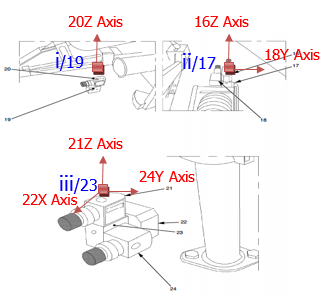
\includegraphics[width=0.6\linewidth]{gambar/peletakan_sensor.png}
	\caption{Peletakan akseleromter pada Helikopter.}
	\label{peletakan_sensor.png}
\end{figure}

\begin{longtable}{|c|c|}
	\caption{Lokasi dan arah akseleromter.}
	\label{tb:lokasiakselero}                        	\\
	\hline
	\textbf{Channel} & \textbf{Lokasi akselerometer} 	\\
	\hline
	1            	 & Kursi pilot (20Z)             	\\
	\hline
	2			     & Bagian luar stik kopilot (16Z)   \\
	\hline
	3				 & Bagian luar stik kopilot	(18Y)   \\
	\hline
	4				 & Frame 9" (21Z)                   \\
	\hline
	5				 & Frame 9" (22X)					\\
	\hline
	6				 & Frame 9" (24Y)					\\
	\hline
\end{longtable}

Kemudian berikut (gambar \ref{tampak_atas.png}, \ref{tampak_depan.png}, \ref{tampak_samping.png}) merupakan skema Helikopter AS 565 MBe Panther yang digunakan beserta keterangan dimensi dari beberapa arah skema.

\begin{figure}[H]
	\centering
	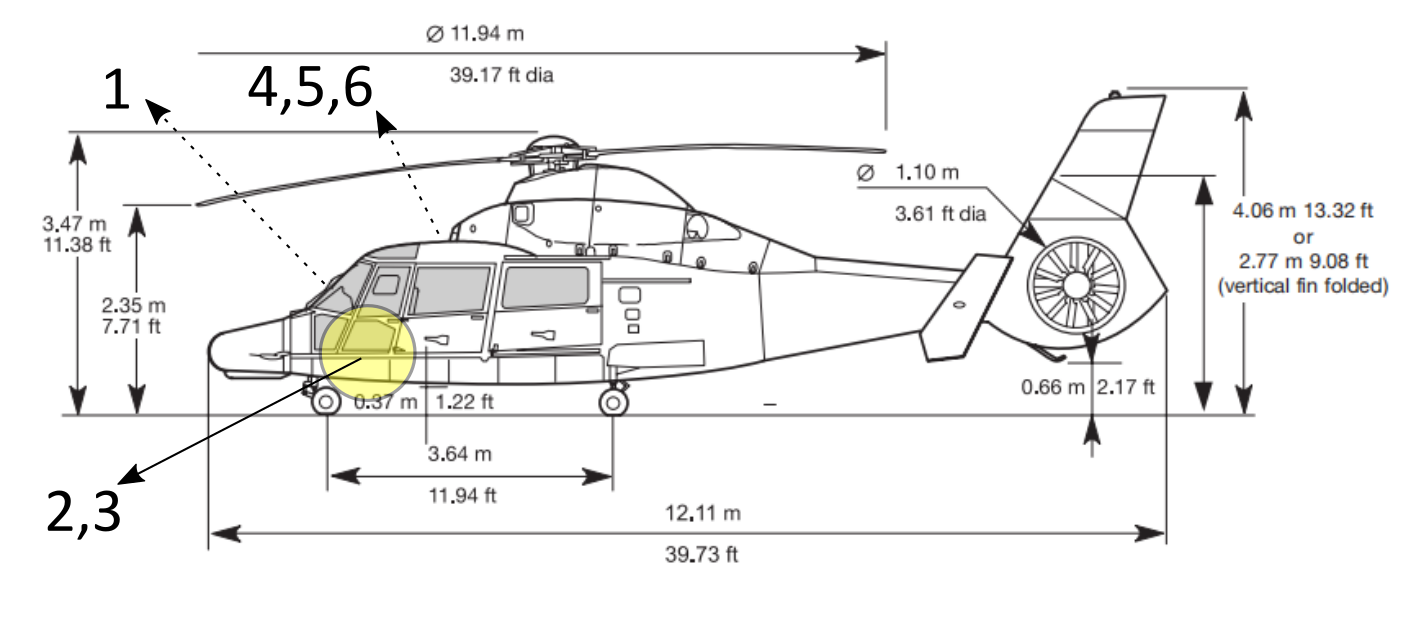
\includegraphics[width=0.8\linewidth]{gambar/tampak_samping.png}
	\caption{Skema penempatan \textit{channel} sensor dan dimensi helikopter AS 565 MBe Panther (tampak samping).}
	\label{tampak_samping.png}
\end{figure}

\begin{figure}[H]
	\centering
	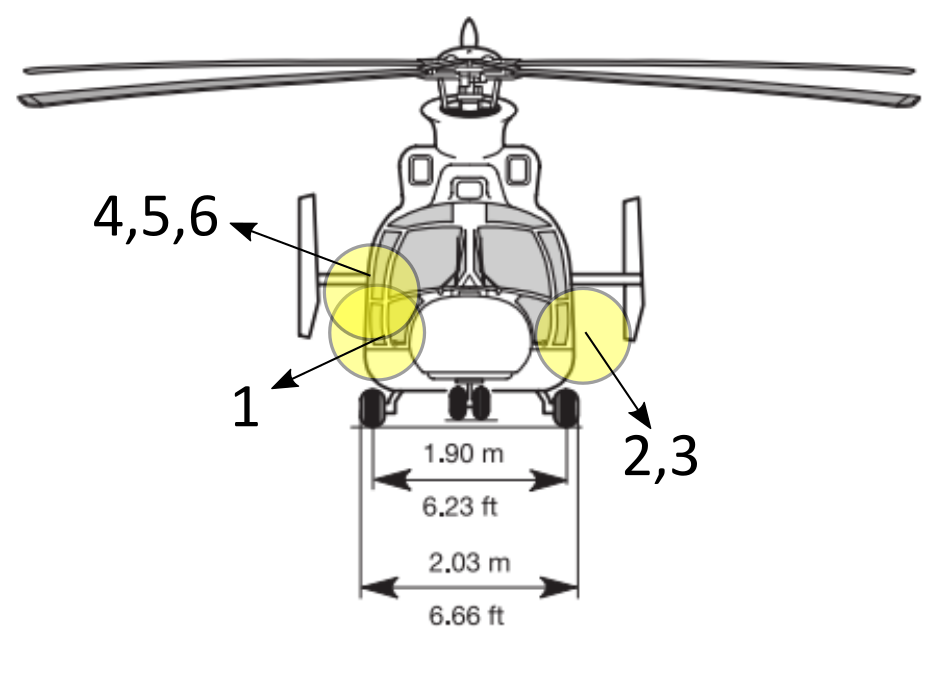
\includegraphics[width=0.6\linewidth]{gambar/tampak_depan.png}
	\caption{Skema penempatan \textit{channel} sensor dan dimensi helikopter AS 565 MBe Panther (tampak depan).}
	\label{tampak_depan.png}
\end{figure}

\begin{figure}[H]
	\centering
	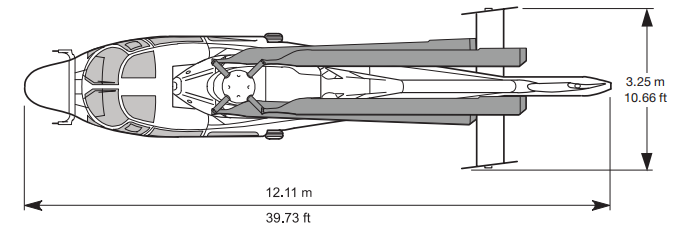
\includegraphics[width=0.75\linewidth]{gambar/tampak_atas.png}
	\caption{Skema penempatan \textit{channel} sensor dan dimensi helikopter AS 565 MBe Panther (tampak atas).}
	\label{tampak_atas.png}
\end{figure}

Tabel \ref{tb:variasilanding} merupakan variasi pada \textit{landing gear absorbers}. Variasi tersebut dilakukan pada bagian ban dan oleo helikopter. Propertis mengenai variasi \textit{landing gear absorbers} ditampilkan pada tabel \ref{tb:propertiskuantitatif}. Selanjutnya pada tabel \ref{tb:variasi_input} memberikan informasi yang berkaitan dengan variasi \textit{input} pada \textit{ground test}. Secara teknis, dalam 1 kondisi pengujian terdapat 12 variasi \textit{input} yang diberikan kepada helikopter.

\begin{table}[H]
	\centering
	\caption{Variasi \textit{Landing gear absorbers.}}
	\label{tb:variasilanding}
	\resizebox{0.7\textwidth}{!}{%
		\begin{tabular}{|c|ccccc|}
			\hline
			\multirow{3}{*}{No} & \multicolumn{5}{c|}{Kondisi pengujian Oleo/Tyre} \\ \cline{2-6} 
			& \multicolumn{1}{c|}{Bagian Depan} & \multicolumn{2}{c|}{Bagian Kiri} & \multicolumn{2}{c|}{Bagian Kanan} \\ \cline{2-6} 
			& \multicolumn{1}{c|}{Oleo/Tyre} & \multicolumn{1}{c|}{Oleo} & \multicolumn{1}{c|}{Tyre} & \multicolumn{1}{c|}{Oleo} & Tyre \\ \hline
			1 & \multicolumn{1}{c|}{Nominal/Nominal} & \multicolumn{1}{c|}{Nominal} & \multicolumn{1}{c|}{Nominal} & \multicolumn{1}{c|}{Nominal} & Nominal \\ \hline
			2 & \multicolumn{1}{c|}{Nominal/Nominal} & \multicolumn{1}{c|}{High} & \multicolumn{1}{c|}{High} & \multicolumn{1}{c|}{Nominal} & Nominal \\ \hline
			3 & \multicolumn{1}{c|}{Nominal/Nominal} & \multicolumn{1}{c|}{Nominal} & \multicolumn{1}{c|}{Nominal} & \multicolumn{1}{c|}{High} & High \\ \hline
			4 & \multicolumn{1}{c|}{Nominal/Nominal} & \multicolumn{1}{c|}{Nominal} & \multicolumn{1}{c|}{Nominal} & \multicolumn{1}{c|}{Low} & Low \\ \hline
			5 & \multicolumn{1}{c|}{Nominal/Nominal} & \multicolumn{1}{c|}{Low} & \multicolumn{1}{c|}{Low} & \multicolumn{1}{c|}{Nominal} & Nominal \\ \hline
			6 & \multicolumn{1}{c|}{Nominal/Nominal} & \multicolumn{1}{c|}{High} & \multicolumn{1}{c|}{High} & \multicolumn{1}{c|}{High} & High \\ \hline
			7 & \multicolumn{1}{c|}{Nominal/Nominal} & \multicolumn{1}{c|}{Low} & \multicolumn{1}{c|}{Low} & \multicolumn{1}{c|}{Low} & Low \\ \hline
			8 & \multicolumn{1}{c|}{Nominal/Nominal} & \multicolumn{1}{c|}{High} & \multicolumn{1}{c|}{High} & \multicolumn{1}{c|}{Low} & Low \\ \hline
			9 & \multicolumn{1}{c|}{Nominal/Nominal} & \multicolumn{1}{c|}{Low} & \multicolumn{1}{c|}{Low} & \multicolumn{1}{c|}{High} & High \\ \hline
			10 & \multicolumn{1}{c|}{Nominal/Nominal} & \multicolumn{1}{c|}{High} & \multicolumn{1}{c|}{High} & \multicolumn{1}{c|}{Nominal} & High \\ \hline
			11 & \multicolumn{1}{c|}{Nominal/Nominal} & \multicolumn{1}{c|}{High} & \multicolumn{1}{c|}{High} & \multicolumn{1}{c|}{Low} & High \\ \hline
		\end{tabular}%
	}
\end{table}

\begin{table}[h]
	\centering
	\caption{Propertis kuantitatif variasi \textit{landing gear absorbers} pada ban dan oleo helikopter.}
	\label{tb:propertiskuantitatif}
	\resizebox{0.75\textwidth}{!}{%
		\begin{tabular}{|c|c|c|l|}
			\hline
			\multirow{3}{*}{NLG} & \multirow{2}{*}{Oleo} & \multirow{2}{*}{Nominal} & Hydraulic: 10 bar (145 psi) \\ \cline{4-4} 
			&  &  & Nitrogen 30$^o$C=42 bar(psi) \\ \cline{2-4} 
			& Tyre & Nominal & 5.5 bar (79.7 psi) \\ \hline
			\multirow{9}{*}{MLG} & \multirow{6}{*}{Oleo} & \multirow{2}{*}{Low} & Hydraulic: 10 bar (145 psi) \\ \cline{4-4} 
			&  &  & Nitrogen 15oC: HP=49.0 bar (711 psi) LP=4.0 bar (59.0 psi) \\ \cline{3-4} 
			&  & \multirow{2}{*}{Nominal} & Hydraulic: 10 bar (145 psi) \\ \cline{4-4} 
			&  &  & Nitrogen 30$^o$C: HP=51.5 bar (747 psi) LP=4.2 bar (61 psi) \\ \cline{3-4} 
			&  & \multirow{2}{*}{High} & Hydraulic: 10 bar (145 psi) \\ \cline{4-4} 
			&  &  & Nitrogen 45$^o$C: HP=54.0 bar (783 psi) LP=4.4 bar (63.82 psi) \\ \cline{2-4} 
			& \multirow{3}{*}{Tyre} & Low & 8.48 bar (123 psi) \\ \cline{3-4} 
			&  & Nominal & 10.8 bar (156.6 psi) \\ \cline{3-4} 
			&  & High & 13.1 bar (190 psi) \\ \hline
		\end{tabular}%
	}
\end{table}

\begin{table}[h]
	\centering
	\caption{Variasi \textit{input} pada ground test Helikopter.}
	\label{tb:variasi_input}
	\resizebox{0.75\textwidth}{!}{%
		\begin{tabular}{|c|c|c|c|c|}
			\hline
			No & SAS & Power & Input Control & Name of Sequence \\ \hline
			1 & \multirow{6}{*}{OFF} & Ground Idle & Longitudinal & FILO \\ \cline{1-1} \cline{3-5} 
			2 &  & Ground Idle & Lateral & FILA \\ \cline{1-1} \cline{3-5} 
			3 &  & Flight Idle (on Ground) & Longitudinal & FFLO \\ \cline{1-1} \cline{3-5} 
			4 &  & Flight Idle (on Ground) & Lateral & FFLA \\ \cline{1-1} \cline{3-5} 
			5 &  & Flight Idle (Light on Wheel) & Longitudinal & FLLO \\ \cline{1-1} \cline{3-5} 
			6 &  & Flight Idle (Light on Wheel) & Lateral & FLLA \\ \hline
			7 & \multirow{6}{*}{ON} & Ground Idle & Longitudinal & NILO \\ \cline{1-1} \cline{3-5} 
			8 &  & Ground Idle & Lateral & NILA \\ \cline{1-1} \cline{3-5} 
			9 &  & Flight Idle (on Ground) & Longitudinal & NFLO \\ \cline{1-1} \cline{3-5} 
			10 &  & Flight Idle (on Ground) & Lateral & NFLA \\ \cline{1-1} \cline{3-5} 
			11 &  & Flight Idle (Light on Wheel) & Longitudinal & NLLO \\ \cline{1-1} \cline{3-5} 
			12 &  & Flight Idle (Light on Wheel) & Lateral & NLLA \\ \hline
		\end{tabular}%
	}
\end{table}

Semua data yang didapatkan pada hasil pengukuran \textit{damping ratio} dan vibrasi oleh akselerometer selanjutnya akan diolah dan dianalisis apakah helikopter AS 565 MBe Panther hasil modifikasi tersebut berpotensi mengalami fenomena \textit{ground resonance}. Sehingga helikopter dapat dikatakan aman untuk dapat digunakan sebagaimana kegunaannya setelah dimodifikasi. Kemudian, data vibrasi pada akselerometer akan dimasukkan pada batas siklus osilasi sesuai dengan acuan yang terdapat di standar MIL-STD-810H-Method-514.8 (vibrasi). Informasi dari standar tersebut dapat dilihat pada tabel \ref{tb:MIL-STD}.

\begin{table}[]
	\centering
	\caption{Tabel acuan MIL-STD-810H-Method-514.8 untuk menghitung batas osilasi yang dimiliki oleh helikopter.}
	\label{tb:MIL-STD}
	\resizebox{\textwidth}{!}{%
		\begin{tabular}{|cccc|}
			\hline
			\multicolumn{1}{|c|}{Materiel} & \multicolumn{1}{c|}{Random Levels} & \multicolumn{1}{c|}{\begin{tabular}[c]{@{}c@{}}Source Frequency ($f_x$)\\ Range (Hz)\end{tabular}} & \begin{tabular}[c]{@{}c@{}}Peak Acceleration ($A_x$) \\ at $f_x$ (Gravity Units (g))\end{tabular} \\ \hline
			\multicolumn{1}{|c|}{\multirow{5}{*}{General}} & \multicolumn{1}{c|}{$W_o = 0.0010 g^2/Hz$} & \multicolumn{1}{c|}{$3 to \leq 10$} & 0.7/(10.70-$f_x$) \\ \cline{2-4} 
			\multicolumn{1}{|c|}{} & \multicolumn{1}{c|}{$W_1 = 0.010 g^2/Hz$} & \multicolumn{1}{c|}{$>10$ to $25$} & 0.10 $f_x$ \\ \cline{2-4} 
			\multicolumn{1}{|c|}{} & \multicolumn{1}{c|}{\multirow{3}{*}{$f_1=500 Hz$}} & \multicolumn{1}{c|}{25 to 40} & 2.5 \\ \cline{3-4} 
			\multicolumn{1}{|c|}{} & \multicolumn{1}{c|}{} & \multicolumn{1}{c|}{40 to 50} & 6.50 - 0.1 $f_x$ \\ \cline{3-4} 
			\multicolumn{1}{|c|}{} & \multicolumn{1}{c|}{} & \multicolumn{1}{c|}{50 to 500} & 1.5 \\ \hline
			\multicolumn{4}{|c|}{Main Rotor Frequencies (Hz)} \\ \hline
			\multicolumn{2}{|c|}{$f_1$ = 1P} & \multicolumn{2}{c|}{Fundamental} \\ \hline
			\multicolumn{2}{|c|}{$f_2$ = n*1P} & \multicolumn{2}{c|}{blade passage (BP)} \\ \hline
			\multicolumn{2}{|c|}{$f_3 = 2f_2$} & \multicolumn{2}{c|}{$2^{nd}$ harmonic} \\ \hline
			\multicolumn{2}{|c|}{$f_4 = 3f_2$} & \multicolumn{2}{c|}{$3^{rd}$ harmonic} \\ \hline
		\end{tabular}%
	}
\end{table}

\section{Pemodelan pada Femap}
	\label{sec:femap}
\subsection{Skema Pemodelan}
Dalam mencari solusi yang secara tepat merepresentasikan batas siklus osilasi pada perhitungan matematis. Berdasarkan referensi yang telah didapatkan, diperlukan langkah awal membuat skema pemodelan sederhana yang selanjutnya akan membantu untuk mendefinisikan posisi pusat massa dari masing-masing rotor pada helikopter. Skema pemodelan ini berdasarkan pada gambar \ref{tampak_atas.png} untuk menggambar bagian helikopter pada bagian tampak atas. Sedangkan gambar \ref{tampak_samping.png}. Skema gambar menggunakan bantuan \textit{software} desain Inkscape untuk memberikan bentuk \textit{node} pada kerangka yang helikopter yang akan digambar. Gambar \ref{fig:skema_model} ini merupakan skema kerangka helikopter untuk memodelkan helikopter dengan bentuk yang sederhana agar nantinya dapat diolah menggunakan prinsip elemen hingga (\textit{finite element}) pada \textit{software} FEMAP.

\begin{figure}[H]
	\centering
	\includegraphics[width=\linewidth]{gambar/rancangan_skema.png}
	\caption{Skema pemodelan helikopter untuk bagian samping, atas, dan bawah.}
	\label{fig:skema_model}
\end{figure}

Koordinat pada helikopter didapatkan dengan menggunakan dimensi yang mendekati ukuran sebenarnya dari helikopter. Oleh karena itu pada gambar \ref{fig:skema_model} digunakan bayangan kerangka helikopter yang sebenarnya dari AS 565 MBe Panther. Rasio yang dimiliki pada skema gambar tersebut adalah 0.0778m/mm, yang artinya dalam setiap panjang 1mm pada gambar, mewakili 0.0778 meter pada dimensi helikopter yang sebenarnya.

\subsection{Penentuan Koordinat}

Selanjutnya, pada gambar \ref{fig:skema_model} akan didefinisikan titik-titik yang nantinya akan menjadi \textit{node} pada kerangka helikopter. Titik-titik tersebut akan didefinisikan dalam koordinat kartesian dalam sumbu-x,y, dan z. Titik 2s', 2s dan 3s' akan menjadi titik diberikannya gaya luar untuk simulasi pada FEMAP. Hal ini dikarenakan pada titik tersebut terdapat sensor akselerometer.


\begin{table}[h]
	\centering
	\caption{Koordinat masing-masing tanda pada titik dalam 3 dimensi.}
	\label{tb:koordinat}
	\resizebox{0.93\textwidth}{!}{%
		\begin{tabular}{|
				>{\columncolor[HTML]{FFCCC9}}c |
				>{\columncolor[HTML]{FFCE93}}c |ccc|
				>{\columncolor[HTML]{FFCCC9}}c |
				>{\columncolor[HTML]{FFCE93}}c |ccc|}
			\hline
			\cellcolor[HTML]{FFCCC9} & \cellcolor[HTML]{FFCE93} & \multicolumn{3}{c|}{Koordinat (m)} & \cellcolor[HTML]{FFCCC9} & \cellcolor[HTML]{FFCE93} & \multicolumn{3}{c|}{Koordinat (m)} \\ \cline{3-5} \cline{8-10} 
			\multirow{-2}{*}{\cellcolor[HTML]{FFCCC9}ID} & \multirow{-2}{*}{\cellcolor[HTML]{FFCE93}Mark} & \multicolumn{1}{c|}{x} & \multicolumn{1}{c|}{y} & z & \multirow{-2}{*}{\cellcolor[HTML]{FFCCC9}ID} & \multirow{-2}{*}{\cellcolor[HTML]{FFCE93}Mark} & \multicolumn{1}{c|}{x} & \multicolumn{1}{c|}{y} & z \\ \hline
			1 & 10s & \multicolumn{1}{c|}{8.4295} & \multicolumn{1}{c|}{0.4676} & 0.3466 & 17 & 4s & \multicolumn{1}{c|}{4.3831} & \multicolumn{1}{c|}{-0.1945} & -0.4085 \\ \hline
			2 & 11s & \multicolumn{1}{c|}{8.8695} & \multicolumn{1}{c|}{0.4806} & 0.3466 & 18 & 4s' & \multicolumn{1}{c|}{4.3831} & \multicolumn{1}{c|}{-0.1945} & 1.1987 \\ \hline
			3 & 12s & \multicolumn{1}{c|}{10.2371} & \multicolumn{1}{c|}{0.6235} & 0.3466 & 19 & 5a & \multicolumn{1}{c|}{1.4013} & \multicolumn{1}{c|}{0.9972} & -0.0374 \\ \hline
			4 & 13s & \multicolumn{1}{c|}{10.2087} & \multicolumn{1}{c|}{1.5276} & 0.3466 & 20 & 5a' & \multicolumn{1}{c|}{1.4013} & \multicolumn{1}{c|}{0.9972} & 0.7295 \\ \hline
			5 & 14s & \multicolumn{1}{c|}{10.9654} & \multicolumn{1}{c|}{3.0033} & 0.3466 & 21 & 5s & \multicolumn{1}{c|}{1.6449} & \multicolumn{1}{c|}{0.9972} & -0.32144 \\ \hline
			6 & 15s & \multicolumn{1}{c|}{11.1567} & \multicolumn{1}{c|}{0.8293} & 0.3466 & 22 & 5s' & \multicolumn{1}{c|}{1.6449} & \multicolumn{1}{c|}{0.9972} & 1.0146 \\ \hline
			7 & 1a & \multicolumn{1}{c|}{3.0017} & \multicolumn{1}{c|}{1.739} & 0.7762 & 23 & 6s & \multicolumn{1}{c|}{2.5934} & \multicolumn{1}{c|}{0.9972} & -0.5704 \\ \hline
			8 & 1a' & \multicolumn{1}{c|}{3.0017} & \multicolumn{1}{c|}{1.739} & -0.0801 & 24 & 7a & \multicolumn{1}{c|}{8.8695} & \multicolumn{1}{c|}{0.4806} & 1.6486 \\ \hline
			9 & 1s & \multicolumn{1}{c|}{0} & \multicolumn{1}{c|}{0} & 0 & 25 & 7a' & \multicolumn{1}{c|}{8.8695} & \multicolumn{1}{c|}{0.4806} & -0.9553 \\ \hline
			10 & 1s' & \multicolumn{1}{c|}{0} & \multicolumn{1}{c|}{0} & 0.6932 & 26 & 7s & \multicolumn{1}{c|}{4.3831} & \multicolumn{1}{c|}{0.9972} & -0.4707 \\ \hline
			11 & 2a' & \multicolumn{1}{c|}{5.3859} & \multicolumn{1}{c|}{1.739} & 0.681 & 27 & 8s & \multicolumn{1}{c|}{2.9028} & \multicolumn{1}{c|}{1.739} & -0.5704 \\ \hline
			12 & 2a & \multicolumn{1}{c|}{5.3859} & \multicolumn{1}{c|}{1.739} & 0.0128 & 28 & 8s' & \multicolumn{1}{c|}{2.9028} & \multicolumn{1}{c|}{1.739} & 1.2081 \\ \hline
			13 & 2s & \multicolumn{1}{c|}{1.019} & \multicolumn{1}{c|}{-0.1945} & -0.4085 & 29 & 9s & \multicolumn{1}{c|}{4.8087} & \multicolumn{1}{c|}{1.739} & -0.4707 \\ \hline
			14 & 2s' & \multicolumn{1}{c|}{1.019} & \multicolumn{1}{c|}{-0.1945} & 1.1987 & 30 & 9s' & \multicolumn{1}{c|}{4.8087} & \multicolumn{1}{c|}{1.739} & 1.1639 \\ \hline
			15 & 3s & \multicolumn{1}{c|}{2.6192} & \multicolumn{1}{c|}{-0.1945} & -0.4085 & 31 & 6s' & \multicolumn{1}{c|}{2.5934} & \multicolumn{1}{c|}{0.9972} & 1.2081 \\ \hline
			16 & 3s' & \multicolumn{1}{c|}{2.6192} & \multicolumn{1}{c|}{-0.1945} & 1.1987 & 32 & 7s' & \multicolumn{1}{c|}{4.3831} & \multicolumn{1}{c|}{0.9972} & 1.1639 \\ \hline
		\end{tabular}%
	}
\end{table}

Tabel \ref{tb:koordinat} merupakan koordinat yang didefinisikan dengan titik acuan berada pada 1s, sehingga titik 1s didefinsikan dengan koordinat x,y, dan z beruturut-turut, 0, 0, dan 0. Setelah koordinat ditentukan, maka pada tahap selanjutnya adalah melakukan pemodelan pada FEMAP untuk selanjutnya nanti akan dilakukan analisis menggunakan nilai eigen untuk mencari \textit{mode shape} pada helikopter. Informasi mengenai \textit{mode shape} ini nantinya akan digunakan untuk memberikan gambaran bahwa helikopter akan memiliki respon sedemikian rupa untuk dapat menjelaskan fenomena \textit{ground resonance} yang berpotensi terjadi pada helikopter.
\cleardoublepage

% Bab 4 pengujian dan analisis
\chapter{HASIL DAN PEMBAHASAN}
\label{chap:hasil dan pembahasan}

% Ubah bagian-bagian berikut dengan isi dari pengujian dan analisis

Pada penelitian ini dilakukan 3 aspek pengerjaan dalam menjawab tujuannya, diantaranya adalah data eksperimen yang telah didapatkan dari PTDI. Kemudian validasi matematis menggunakan landasan teori yang telah disesuaikan dengan kondisi pengerjaan penelitian ini, yaitu \textit{ground resonance} helikopter. Kemudian yang terakhir adalah simulasi untuk mendukung hasil data pengukuran dan perhitungan. 

\section{Hasil pengukuran getaran pada FTIS}

Hasil pengukuran data \textit{ground test} dibagi menjadi 2 bagian, seperti yang telah dijelaskan pada bagian metodologi penelitian, bahwa data yang didapatkan merupakan data pengukuran getaran pada FTIS untuk mencari \textit{damping ratio} dan pengukuran data getaran pada akseleromter untuk mendapatkan respon frekuensi dominan oleh helikopter akibat \textit{input} yang diberikan. Berikut ini merupakan grafik yang didapatkan dari masing-masing kondisi yang mengacu pada tabel \ref{tb:variasilanding}.

\begin{figure}[H]
	\centering
	\fbox{\includegraphics[width=0.7\linewidth]{gambar/FTIS_image/All-plot/All_config_1.jpg}}
	\caption{Grafik data hasil pengukuran kondisi 1.}
	\label{fig:condition_1}
\end{figure}

Selanjutnya merupakan grafik dengan keterangan serupa, dimana pada grafik tersebut memiliki keterangan sebagaimana pada tabel berikut:

\begin{table}[]
	\caption{Keterangan pengukuran pada grafik}
	\begin{tabular}{|c|c|c|}
		\hline
		\textit{Lateral cyclic displacement (\%)} & \textit{Longitudinal cyclic displacement} & Pedal displacement (\%)           \\ \hline
		\textit{Roll (deg)}                       & \textit{Pitch (deg)}                      & \textit{Heading (deg)}            \\ \hline
		\textit{Rate of roll (deg/s)}             & \textit{Rate of Pitch (deg/s)}            & \textit{Rate of Yaw (deg/s)}      \\ \hline
		\textit{Acceleration-x ($m/s^2$)}         & \textit{Acceleration-y ($m/s^2$)}         & \textit{Acceleration-z ($m/s^2$)} \\ \hline
	\end{tabular}
\end{table}

Posisi dari masing-masing keterangan berkorelasi dengan posisi pada grafik yang diberikan, contoh: pada bagian awal, dari arah kiri terdapat keterangan "\textbf{\textit{Lateral Cyclic Displacement (\%)}}" maka grafik pada posisi tersebut merepresentasikan "\textbf{\textit{Lateral Cyclic Displacement (\%)}}", begitu seterusnya.

\begin{figure}[H]
	\centering
	\begin{subfigure}{0.49\textwidth}
		\centering
		\fbox{\includegraphics[width=0.9\linewidth]{gambar/FTIS_image/All-plot/All_config_2.jpg}}
		\caption{}
		\label{fig:condition_2}
	\end{subfigure}
	\centering
	\begin{subfigure}{0.49\textwidth}
		\centering
		\fbox{\includegraphics[width=0.9\linewidth]{gambar/FTIS_image/All-plot/All_config_3.jpg}}
		\caption{}
		\label{fig:condition_3}
	\end{subfigure}
	\caption{(a) Grafik data pengukuran pada kondisi-2 (b) Grafik data pengukuran pada kondisi-3.}
\end{figure}

\begin{figure}[H]
	\begin{subfigure}{0.49\textwidth}
		\centering
		\fbox{\includegraphics[width=0.9\linewidth]{gambar/FTIS_image/All-plot/All_config_4.jpg}}
		\caption{}
		\label{fig:condition_4}
	\end{subfigure}
	\centering
	\begin{subfigure}{0.49\textwidth}
		\centering
		\fbox{\includegraphics[width=0.9\linewidth]{gambar/FTIS_image/All-plot/All_config_5.jpg}}
		\caption{}
		\label{fig:condition_5}
	\end{subfigure}
	\caption{(a) Grafik data pengukuran pada kondisi-4 (b) Grafik data pengukuran pada kondisi-5.}
\end{figure}

\begin{figure}[H]
	\begin{subfigure}{0.49\textwidth}
		\centering
		\fbox{\includegraphics[width=0.9\linewidth]{gambar/FTIS_image/All-plot/All_config_6.jpg}}
		\caption{}
		\label{fig:condition_6}
	\end{subfigure}
	\centering
	\begin{subfigure}{0.49\textwidth}
		\centering
		\fbox{\includegraphics[width=0.9\linewidth]{gambar/FTIS_image/All-plot/All_config_7.jpg}}
		\caption{}
		\label{fig:condition_7}
	\end{subfigure}
	\caption{(a) Grafik data pengukuran pada kondisi-6 (b) Grafik data pengukuran pada kondisi-7.}
\end{figure}

\begin{figure}[H]
	\begin{subfigure}{0.49\textwidth}
		\centering
		\fbox{\includegraphics[width=0.9\linewidth]{gambar/FTIS_image/All-plot/All_config_8.jpg}}
		\caption{}
		\label{fig:condition_8}
	\end{subfigure}
	\centering
	\begin{subfigure}{0.49\textwidth}
		\centering
		\fbox{\includegraphics[width=0.9\linewidth]{gambar/FTIS_image/All-plot/All_config_9.jpg}}
		\caption{}
		\label{fig:condition_9}
	\end{subfigure}
	\caption{(a) Grafik data pengukuran pada kondisi-8 (b) Grafik data pengukuran pada kondisi-9.}
\end{figure}

\begin{figure}[H]
	\begin{subfigure}{0.49\textwidth}
		\centering
		\fbox{\includegraphics[width=0.9\linewidth]{gambar/FTIS_image/All-plot/All_config_10.jpg}}
		\caption{}
		\label{fig:condition_10}
	\end{subfigure}
	\centering
	\begin{subfigure}{0.49\textwidth}
		\centering
		\fbox{\includegraphics[width=0.9\linewidth]{gambar/FTIS_image/All-plot/All_config_11.jpg}}
		\caption{}
		\label{fig:condition_11}
	\end{subfigure}
	\caption{(a) Grafik data pengukuran pada kondisi-10 (b) Grafik data pengukuran pada kondisi-11.}
\end{figure}

\begin{table}[H]
	\centering
	\caption{Hasil identifikasi damping ratio rata-rata dari respon helikopter berdasarkan variasi kondisi}
	\label{tb:damp_ratio_table}
	\resizebox{\textwidth}{!}{%
		\begin{tabular}{|c|ccccccccc|}
			\hline
			\multirow{2}{*}{Kondisi} & \multicolumn{9}{c|}{Rata-rata \textit{damping ratio} respon} \\ \cline{2-10} 
			& \multicolumn{1}{c|}{Roll} & \multicolumn{1}{c|}{Pitch} & \multicolumn{1}{c|}{Heading} & \multicolumn{1}{c|}{Rate of Roll} & \multicolumn{1}{c|}{Rate of Pitch} & \multicolumn{1}{c|}{Rate of Yaw} & \multicolumn{1}{c|}{Acceleration-X} & \multicolumn{1}{c|}{Acceleration-Y} & Acceleration-Z \\ \hline
			1 & \multicolumn{1}{c|}{-} & \multicolumn{1}{c|}{-} & \multicolumn{1}{c|}{-} & \multicolumn{1}{c|}{0.05285435} & \multicolumn{1}{c|}{0.036747763} & \multicolumn{1}{c|}{-} & \multicolumn{1}{c|}{-} & \multicolumn{1}{c|}{0.050426643} & - \\ \hline
			2 & \multicolumn{1}{c|}{-} & \multicolumn{1}{c|}{-} & \multicolumn{1}{c|}{-} & \multicolumn{1}{c|}{0.058120539} & \multicolumn{1}{c|}{-} & \multicolumn{1}{c|}{0.045805814} & \multicolumn{1}{c|}{-} & \multicolumn{1}{c|}{0.038387333} & - \\ \hline
			3 & \multicolumn{1}{c|}{-} & \multicolumn{1}{c|}{-} & \multicolumn{1}{c|}{-} & \multicolumn{1}{c|}{0.055225124} & \multicolumn{1}{c|}{0.05507518} & \multicolumn{1}{c|}{0.043144563} & \multicolumn{1}{c|}{-} & \multicolumn{1}{c|}{0.040316101} & - \\ \hline
			4 & \multicolumn{1}{c|}{-} & \multicolumn{1}{c|}{-} & \multicolumn{1}{c|}{-} & \multicolumn{1}{c|}{0.055248847} & \multicolumn{1}{c|}{0.04408422} & \multicolumn{1}{c|}{0.036747763} & \multicolumn{1}{c|}{-} & \multicolumn{1}{c|}{0.062462147} & - \\ \hline
			5 & \multicolumn{1}{c|}{-} & \multicolumn{1}{c|}{-} & \multicolumn{1}{c|}{-} & \multicolumn{1}{c|}{0.064958942} & \multicolumn{1}{c|}{0.054761252} & \multicolumn{1}{c|}{-} & \multicolumn{1}{c|}{-} & \multicolumn{1}{c|}{0.035288539} & - \\ \hline
			6 & \multicolumn{1}{c|}{-} & \multicolumn{1}{c|}{-} & \multicolumn{1}{c|}{-} & \multicolumn{1}{c|}{0.050658456} & \multicolumn{1}{c|}{0.04408422} & \multicolumn{1}{c|}{-} & \multicolumn{1}{c|}{-} & \multicolumn{1}{c|}{0.064120389} & - \\ \hline
			7 & \multicolumn{1}{c|}{-} & \multicolumn{1}{c|}{-} & \multicolumn{1}{c|}{-} & \multicolumn{1}{c|}{0.04732238} & \multicolumn{1}{c|}{0.043670692} & \multicolumn{1}{c|}{0.047821495} & \multicolumn{1}{c|}{-} & \multicolumn{1}{c|}{0.064757723} & - \\ \hline
			8 & \multicolumn{1}{c|}{-} & \multicolumn{1}{c|}{-} & \multicolumn{1}{c|}{-} & \multicolumn{1}{c|}{0.049504081} & \multicolumn{1}{c|}{0.05727551} & \multicolumn{1}{c|}{-} & \multicolumn{1}{c|}{-} & \multicolumn{1}{c|}{0.048365129} & - \\ \hline
			9 & \multicolumn{1}{c|}{-} & \multicolumn{1}{c|}{-} & \multicolumn{1}{c|}{-} & \multicolumn{1}{c|}{-} & \multicolumn{1}{c|}{-} & \multicolumn{1}{c|}{-} & \multicolumn{1}{c|}{-} & \multicolumn{1}{c|}{-} & - \\ \hline
			10 & \multicolumn{1}{c|}{-} & \multicolumn{1}{c|}{-} & \multicolumn{1}{c|}{-} & \multicolumn{1}{c|}{-} & \multicolumn{1}{c|}{-} & \multicolumn{1}{c|}{-} & \multicolumn{1}{c|}{-} & \multicolumn{1}{c|}{-} & - \\ \hline
			11 & \multicolumn{1}{c|}{-} & \multicolumn{1}{c|}{-} & \multicolumn{1}{c|}{-} & \multicolumn{1}{c|}{-} & \multicolumn{1}{c|}{-} & \multicolumn{1}{c|}{-} & \multicolumn{1}{c|}{-} & \multicolumn{1}{c|}{-} & - \\ \hline
			Rata-rata total & \multicolumn{1}{c|}{-} & \multicolumn{1}{c|}{-} & \multicolumn{1}{c|}{-} & \multicolumn{1}{c|}{0.05423659} & \multicolumn{1}{c|}{0.047956977} & \multicolumn{1}{c|}{0.043379909} & \multicolumn{1}{c|}{-} & \multicolumn{1}{c|}{0.050515501} & - \\ \hline
		\end{tabular}%
	}
\end{table}

Pada grafik diatas dibagi menjadi beberapa segmen yang sesuai dengan variasi \textit{input} yang telah diberikan pada tabel \ref{tb:variasi_input} sehingga selanjutnya akan dihitung nilai \textit{damping ratio} dari masing-masing orientasi respon helikopter. \textit{Damping ratio} pada respon helikopter akan dihitung setelah helikopter berhenti memberikan \textit{input}. Sehingga didapatkan tabel \ref{tb:damp_ratio_table} yang memberikan informasi hasil perhitungan \textit{damping ratio} pada helikopter.

Data pengukuran getaran yang didapatkan dari FTIS merupakan data yang diidentifikasi untuk melihat potensi terjadinya \textit{ground resonance} secara visual. Apabila terdapat respon yang meningkat setelah \textit{input} berhenti, maka berdasarkan teori yang telah dijelaskan pada fenomena \textit{ground resonance}. Kondisi tersebut merupakan kondisi awal mula terjadinya \textit{self-excited} yang membuat kerangka helikopter bergetar dengan amplitudo yang semakin besar, sehingga helikopter mengalami kerusakan. Dari variasi \textit{input} yang telah dijelaskan, \textit{input} hanya berasal dari \textit{longitudinal cyclic displacement} dan \textit{lateral cyclic displacement}. Pada gambar \ref{fig:condition_1} hingga \ref{fig:condition_11} dapat dilihat bahwa setiap \textit{input} memiliki respon pada setiap orientasi helikopter, dimulai dari \textit{roll, pitch, heading, rate of roll, rate of pitch, rate of yaw,} percepatan pada arah-X,Y, dan Z. 

Dari tabel \ref{tb:damp_ratio_table} didapatkan informasi bahwa hanya pada orientasi \textit{rate of roll, rate of pitch, rate of yaw,} dan percepatan pada arah sumbu-Y yang dapat diidentifikasi untuk menghitung \textit{damping ratio} helikopter. Hal ini menandakan bahwa helikopter memiliki respon untuk goncangan kanan dan kiri (\textit{rate of roll}) pada tumpuan bannya dengan \textit{damping ratio} rata-rata sebesar 0.054. Respon yang selanjutnya juga memberikan nilai setelah \textit{input} berhenti adalah pada bagian \textit{rate of pitch}, hal ini menandakan bahwa helikopter juga mengalami guncangan ke arah depan dan belakang dengan \textit{damping ratio} rata-rata sebesar 0.0479. Kemudian pada respon \textit{rate of yaw} didapatkan besaran \textit{damping ratio} rata-rata sebesar 0.0433 dan respon percepatan pada arah sumbu-Y dengan \textit{damping ratio} sebesar 0.0505. Hal ini memberikan informasi bahwa helikopter juga memiliki kecenderungan untuk bergerak dengan orientasi arah ke-kanan dan kiri, namun respon tersebut tidak sebanyak dan sebesar pada respon \textit{rate of roll}.

Nilai rata-rata \textit{damping ratio} terbesar diberikan oleh \textit{rate of roll} dan respon percepatan pada arah sumbu-Y. Hal ini berkorelasi dengan orientasi helikopter pada gambar \ref{fig:orientasiheli}. Getaran akan lebih sering terjadi pada arah kanan dan kiri. Secara teori, hal ini disebabkan oleh gaya sentrifugal pada rotor. Disisi lain, orientasi perubahan arah \textit{pitch} rotor juga berubah pada saat bilah pada bilah rotor berada tepat pada bagian kiri dan kanan helikopter.

\begin{figure}[H]
	\centering
	\fbox{\includegraphics[width=0.7\linewidth]{gambar/contoh_grafik_damp_ratio.jpg}}
	\caption{Grafik data pengukuran saat respon masih bergetar pada NLLO kondisi-4.}
	\label{fig:NLLO-4}
\end{figure}

\begin{figure}[h]
	\centering
	\fbox{\includegraphics[width=0.7\linewidth]{gambar/Contoh_TC_Config_3_mark10_FLLO.jpg}}
	\caption{Grafik data pengukuran saat respon teredam dengan cepat pada FLLO kondisi-3.}
	\label{fig:FLLO-3_mark10}
\end{figure}

Hasil perhitungan \textit{damping ratio} pada tabel \ref{tb:damp_ratio_table} didapatkan dengan cara melakukan identifikasi melalui data yang telah di-plot seperti pada gambar \ref{fig:NLLO-4} secara visual, yaitu dengan memberikan tanda pada puncak amplitudo hingga amplitudo terendah, kemudian menghitung besarnya \textit{logarithmic decrement} untuk mendapatkan \textit{damping ratio}. Disisi lain terdapat respon yang langsung teredam setelah \textit{input} berhenti, kondisi ini dapat dilihat pada gambar \ref{fig:FLLO-3_mark10}.

\begin{figure}[h]
	\centering
	\fbox{\includegraphics[width=0.5\linewidth]{gambar/Damping_ratio_plot_ROR.jpg}}
	\caption{Grafik nilai \textit{damping ratio} dari \textit{rate of roll} berdasarkan variasi kondisi.}
	\label{fig:plot_ROR}
\end{figure}

\begin{figure}[H]
	\centering
	\fbox{\includegraphics[width=0.5\linewidth]{gambar/Damping_ratio_plot_ROP.jpg}}
	\caption{Grafik nilai \textit{damping ratio} dari \textit{rate of pitch} berdasarkan variasi kondisi.}
	\label{fig:plot_ROP}
\end{figure}

\begin{figure}[h]
	\centering
	\fbox{\includegraphics[width=0.5\linewidth]{gambar/Damping_ratio_plot_ROY.jpg}}
	\caption{Grafik nilai \textit{damping ratio} dari \textit{rate of yaw} berdasarkan variasi kondisi.}
	\label{fig:plot_ROY}
\end{figure}

\begin{figure}[h]
	\centering
	\fbox{\includegraphics[width=0.5\linewidth]{gambar/Damping_ratio_plot_Acc_y.jpg}}
	\caption{Grafik nilai \textit{damping ratio} dari \textit{acceleration-Y} berdasarkan variasi kondisi.}
	\label{fig:plot_Acc_Y}
\end{figure}

\begin{figure}[H]
	\centering
	\fbox{\includegraphics[width=0.5\linewidth]{gambar/All_damping_ratio.jpg}}
	\caption{Grafik nilai \textit{damping ratio} dari keseluruhan respon helikopter berdasarkan variasi kondisi.}
	\label{fig:plot_All}
\end{figure}

Gambar dari \ref{fig:plot_ROR} hingga \ref{fig:plot_Acc_Y} merupakan plot nilai \textit{damping ratio} berdasarkan masing-masing kondisi untuk orientasi \textit{rate of roll, rate of pitch, rate of yaw,} dan percepatan dalam arah sumbu-Y. Sumbu-x pada gambar tersebut merupakan keterangan pada kondisi ke-berapa terdapat \textit{damping ratio} dengan nilai-nilai yang didapatkan dari perhitungan. Pada gambar \ref{fig:plot_ROR} \textit{damping ratio} tertinggi pada respon \textit{rate of roll} berada pada nilai 0.0912 di kondisi-5 dan terendah pada nilai 0.0291 di kondisi-6. Sedangkan pada gambar \ref{fig:plot_ROP} memberikan informasi nilai \textit{damping ratio} pada \textit{rate of pitch} terbesar pada nilai 0.0572 yang terjadi pada kondisi-8 dan terkecil pada nilai 0.0367 yang terjadi di kondisi-1. Selanjutnya pada gambar \ref{fig:plot_ROY} didapatkan nilai \textit{damping ratio} terbesar pada nilai 0.0478 di kondisi-7 dan terkecil pada nilai 0.0367 di kondisi-4. Kemudian pada arah sumbu-Y, didapatkan nilai \textit{damping ratio} terbesar pada nilai 0.0647 di kondisi-7 dan terkecil pada 0.0352 di kondisi-5.  

Saat pengujian, helikopter memberikan respon getaran yang normal, namun kuantifikasi terhadap kondisi tersebut belum menjelaskan seberapa aman helikopter tersebut dari fenomena \textit{ground resonance}. Perhitungan \textit{damping ratio} setidaknya menjelaskan respon yang dimiliki oleh helikopter terhadap orientasi gerakannya di tanah. Meskipun secara visual, respon helikopter secara jelas tidak menunjukkan adanya potensi terjadinya \textit{ground resonance}. Sehingga identifikasi akan dilanjutkan melalui data hasil pengukuran menggunakan akselerometer.

\section{Hasil pengukuran getaran pada Akselerometer}

Data yang didapatkan dari hasil sensor akselerometer ditunjukkan pada gambar dibawah ini:

\begin{figure}[h]
	\centering
	\fbox{\includegraphics[width=0.7\linewidth]{gambar/raw_config2_ch1.png}}
	\caption{Grafik data pengukuran pada variasi FILO kondisi-2 \textit{channel} 1.}
	\label{fig:raw_config2_FILO}
\end{figure}

\begin{figure}[H]
	\centering
	\fbox{\includegraphics[width=0.7\linewidth]{gambar/fft_config2_ch1.png}}
	\caption{Grafik data hasil FFT pada variasi FILO kondisi-2.}
	\label{fig:fft_config2_FILO}
\end{figure}

Grafik pada gambar \ref{fig:raw_config2_FILO} merupakan grafik data hasil pengukuran yang didapatkan oleh sensor akselerometer pada \textit{channel} 1 dan grafik pada \ref{fig:fft_config2_FILO} merupakan grafik data yang telah diolah menggunakan FFT, sehingga didapatkan nilai dalam domain frekuensi. Data hasil pengukuran menggunakan akselerometer pada gambar diatas akan dibandingkan dengan acuan dari MIL-STD-810H-Method-514.8 (vibrasi). Informasi dari grafik gambar \ref{fig:MIL_STD} didapatkan batas siklus osilasi helikopter. Sehingga didapatkan grafik batas siklus osilasi pada gambar \ref{fig:batas_siklus}.

\begin{figure}[h]
	\centering
	\fbox{\includegraphics[width=0.55\linewidth]{gambar/Oscillation_cycle_limit.jpg}}
	\caption{Grafik batas siklus osilasi dari acuan MIL-STD-810H-Method-514.8 (vibrasi).}
	\label{fig:batas_siklus}
\end{figure}

\begin{table}[H]
	\caption{Tabel perhitungan batas siklus osilasi.}
	\label{tb:batas_siklus}
	\centering
	\begin{tabular}{|ccc|cc|}
		\hline
		\multicolumn{3}{|c|}{Frekuensi (Hz)}                                                       & \multicolumn{2}{c|}{Peak (g)}             \\ \hline
		\multicolumn{1}{|c|}{$f_1$ lower} & \multicolumn{1}{c|}{5.92}  & \multirow{2}{*}{$1p$}       & \multicolumn{1}{c|}{$A_1$ lower} & 0.1464 \\ \cline{1-2} \cline{4-5} 
		\multicolumn{1}{|c|}{$f_1$ upper} & \multicolumn{1}{c|}{6.08}  &                           & \multicolumn{1}{c|}{$A_1$ upper} & 0.1515 \\ \hline
		\multicolumn{1}{|c|}{$f_2$ lower} & \multicolumn{1}{c|}{23.68} & \multirow{2}{*}{$1p*n$}   & \multicolumn{1}{c|}{$A_2$ lower} & 2.368  \\ \cline{1-2} \cline{4-5} 
		\multicolumn{1}{|c|}{$f_2$ upper} & \multicolumn{1}{c|}{24.32} &                           & \multicolumn{1}{c|}{$A_2$ upper} & 2.432  \\ \hline
		\multicolumn{1}{|c|}{$f_3$ lower} & \multicolumn{1}{c|}{47.36} & \multirow{2}{*}{$1p*n*2$} & \multicolumn{1}{c|}{$A_3$ lower} & 1.764 \\ \cline{1-2} \cline{4-5} 
		\multicolumn{1}{|c|}{$f_3$ upper} & \multicolumn{1}{c|}{48.64} &                           & \multicolumn{1}{c|}{$A_3$ upper} & 1.636  \\ \hline
		\multicolumn{1}{|c|}{$f_4$ lower} & \multicolumn{1}{c|}{71.04} & \multirow{2}{*}{$1p*n*3$} & \multicolumn{1}{c|}{$A_4$ lower} & 1.5    \\ \cline{1-2} \cline{4-5} 
		\multicolumn{1}{|c|}{$f_4$ upper} & \multicolumn{1}{c|}{72.96} &                           & \multicolumn{1}{c|}{$A_4$ upper} & 1.5    \\ \hline
	\end{tabular}
\end{table}

Untuk mendapatkan grafik pada gambar \ref{fig:batas_siklus} diperlukan informasi kecepatan rotor helikopter. Diketahui (informasi \textit{flight manual} dari PTDI) nilai kecepatan maksimum dan minimum dari rotor berturut-turut adalah sebesar $365 rpm$ dan $355 rpm$, sehingga didapatkan frekuensi ($f_1$) nya dimulai dari 5.92Hz (minimum) hingga 6.08Hz (maksimum). Perhitungan nilai $f_2$, $f_3$, dan $f_4$ dapat dilihat pada tabel \ref{tb:batas_siklus}. Nilai peak pada tabel tersebut dihitung menggunakan formulasi pada gambar \ref{fig:MIL_STD} yang terletak pada kolom "\textbf{PEAK ACCELERATION ($A_x$) at $f_x$ (GRAVITY UNITS (g))}". Apabila respon sensor akselerometer memiliki nilai frekuensi yang berada diantara batas siklus osilasi dengan amplitudo yang tinggi, maka helikopter memiliki potensi mengalami fenomena \textit{ground resonance} pada frekuensi tersebut. Namun, dari respon yang diberikan oleh helikopter pada semua variasi kondisi dan \textit{input} nilai puncak tertinggi yang dimiliki oleh respon helikopter hanya berada pada nilai 0.143 pada frekuensi 23.68 hingga 24.32 Hz. Sehingga, dari grafik pada gambar \ref{fig:11_FLLO} (kondisi-11 variasi FLLO) tidak ditemukan potensi adanya \textit{ground resonance} pada helikopter. Adapun respon pada kondisi yang lain dengan variasi \textit{input} yang telah ditentukan, responnya memiliki nilai yang lebih kecil dari kondisi pada gambar \ref{fig:11_FLLO}, meskipun respon tersebut berada pada batas siklus osilasi helikopter.

\begin{figure}[h]
	\centering
	\fbox{\includegraphics[width=0.55\linewidth]{gambar/Helicopter_response_GVT_image/Config_11/5_Config_11_FLLO.jpg}}
	\caption{Hasil pengukuran respon frekuensi kondisi-11 pada variasi FLLO pada detik 1800-1850.}
	\label{fig:11_FLLO}
\end{figure}

Grafik pada gambar \ref{fig:11_FLLO} merupakan contoh grafik dengan nilai respon terbesar dibandingkan respon-respon dari kondisi dan variasi lainnya, yaitu dengan amplitudo sebesar 0.143 g-peak pada frekuensi 23.74Hz. Nilai respon yang diberikan pada grafik tersebut merupakan nilai yang didapatkan dari \textit{channel} 1 hingga 6. Data respon yang diberi tanda 'x' merupakan nilai tertinggi dari grafik FFT yang telah didapatkan. Selanjutnya akan coba diidentifikasi bagaimana respon helikopter pada masing-masing \textit{channel} dari kondisi 1 hingga 11.

\begin{figure}[h]
	\centering
	\fbox{\includegraphics[width=0.55\linewidth]{gambar/Plot_per_channel_FTIS/all_channel_1.jpg}}
	\caption{Hasil pengukuran respon frekuensi pada \textit{channel} 1 untuk semua kondisi.}
	\label{fig:channel_1}
\end{figure}

\begin{figure}[h]
	\centering
	\fbox{\includegraphics[width=0.55\linewidth]{gambar/Plot_per_channel_FTIS/all_channel_2.jpg}}
	\caption{Hasil pengukuran respon frekuensi pada \textit{channel} 2 untuk semua kondisi.}
	\label{fig:channel_2}
\end{figure}

\begin{figure}[h]
	\centering
	\fbox{\includegraphics[width=0.55\linewidth]{gambar/Plot_per_channel_FTIS/all_channel_3.jpg}}
	\caption{Hasil pengukuran respon frekuensi pada \textit{channel} 3 untuk semua kondisi.}
	\label{fig:channel_3}
\end{figure}

\begin{figure}[H]
	\centering
	\fbox{\includegraphics[width=0.55\linewidth]{gambar/Plot_per_channel_FTIS/all_channel_4.jpg}}
	\caption{Hasil pengukuran respon frekuensi pada \textit{channel} 4 untuk semua kondisi.}
	\label{fig:channel_4}
\end{figure}

\begin{figure}[H]
	\centering
	\fbox{\includegraphics[width=0.55\linewidth]{gambar/Plot_per_channel_FTIS/all_channel_5.jpg}}
	\caption{Hasil pengukuran respon frekuensi pada \textit{channel} 5 untuk semua kondisi.}
	\label{fig:channel_5}
\end{figure}

\begin{figure}[H]
	\centering
	\fbox{\includegraphics[width=0.55\linewidth]{gambar/Plot_per_channel_FTIS/all_channel_6.jpg}}
	\caption{Hasil pengukuran respon frekuensi pada \textit{channel} 6 untuk semua kondisi.}
	\label{fig:channel_6}
\end{figure}

\begin{table}[H]
	\centering
	\caption{Kuantifikasi banyaknya respon oleh Helikopter pada batas siklus osilasi.}
	\label{tb:identifikasi_pada_batas_siklus}
	\resizebox{\textwidth}{!}{%
		\begin{tabular}{|c|c|c|c|}
			\hline
			Batas siklus & Banyaknya respon (n) & Banyaknya respon (\%) & Total Respon dari (0-80Hz) \\ \hline
			$f_1$ & 0 & 0 & \multirow{4}{*}{2412} \\ \cline{1-3}
			$f_2$ & 383 & 15.87893864 &  \\ \cline{1-3}
			$f_3$ & 103 & 4.270315091 &  \\ \cline{1-3}
			$f_4$ & 15 & 0.621890547 &  \\ \hline
		\end{tabular}%
	}
\end{table}

Grafik pada gambar \ref{fig:channel_1} hingga \ref{fig:channel_6} memberikan informasi terkait respon helikopter dari \textit{channel} 1 hingga 6 untuk semua kondisi. Respon helikopter bertanda 'x' dan diberi warna hijau. Respon tersebut lebih banyak terdapat pada sekitar batas siklus di $f_1$ dan $f_2$. Akan tetapi bila ditinjau secara matematis, tidak terdapat respon helikopter yang berada pada batas siklus $f_1$ hal ini dibuktikan dengan identifikasi nilai kuantitatif respon pada interval $f_1$ seperti yang terdapat pada tabel \ref{tb:identifikasi_pada_batas_siklus}. Dari tabel tersebut, terdapat sebanyak 15.87$\%$ respon helikopter pada batas siklus $f_2$, 4.27$\%$ pada batas siklus $f_3$ dan 0.621$\%$ pada batas siklus $f_4$. Nilai terdekat pada batas siklus $f_1$ berada pada nilai respon frekuensi 5.9166 dan berada pada g-peak 0.0067. Informasi tersebut didapatkan dari data excel yang berjumlah 4539 respon data oleh helikopter seperti yang dapat dilihat pada potongan tabel \ref{tb:list_all_data_sort}. Data yang ditampilkan dan dimasukkan pada batas siklus osilasi hanya merupakan data yang berada pada interval 0 hingga 80Hz. Meskipun pada dasarnya apabila mengacu pada nilai puncak FFT seperti pada gambar \ref{fig:fft_config2_FILO}, didapatkan nilai puncak tertinggi pada rentang frekuensi 700-800Hz.

Identifikasi pada respon frekuensi yang berada di batas siklus osilasi $f_1$ memiliki korelasi yang sangat berkaitan erat dengan fenomena \textit{ground resonance}. Batas siklus osilasi $f_1$ merupakan batas siklus osilasi paling rendah yang berada pada rentang \textit{low frequency}. Berdasarkan penelitian yang telah dikerjakan oleh \cite{Eckert2007AnalyticalAA}, terdapat satu frekuensi pada \textit{lag mode} berupa \textit{low frequency} (frekuensi rendah) yang dapat menyebabkan terjadinya \textit{ground resonance}. Pada rentang frekuensi rendah ini akan dilakukan identifikasi secara matematis sebagai bentuk validasi dari pengukuran data yang telah dilakukan.

\begin{table}[h]
	\centering
	\caption{Tabel respon helikopter pada semua channel dan semua kondisi (potongan).}
	\label{tb:list_all_data_sort}
		\begin{tabular}{|c|c|c|c|}
			\hline
			No & Frekuensi & g-Peak & Channel \\ \hline
			1 & 1.930925 & 0.00063 & ch1 \\ \hline
			2 & 4.869472 & 0.000965 & ch1 \\ \hline
			3 & 7.466667 & 0.000198 & ch1 \\ \hline
			4 & 10.461628 & 0.000213 & ch1 \\ \hline
			5 & 13.358655 & 0.000102 & ch1 \\ \hline
			... & ... & ... & ... \\ \hline
			671 & 5.916678 & 0.006792 & ch2 \\ \hline
			... & ... & ... & ... \\ \hline
			4535 & 1.7132 & 0.01659 & ch6 \\ \hline
			4536 & 1.7683 & 0.01962 & ch6 \\ \hline
			4537 & 1.82582 & 0.02096 & ch6 \\ \hline
			4538 & 23.7427 & 0.02117 & ch6 \\ \hline
			4539 & 746.644 & 0.01644 & ch6 \\ \hline
		\end{tabular}%
\end{table}

\section{Hasil Perhitungan Matematis}

Perhitungan matematis yang dilakukan berdasarkan pada apa yang telah dikerjakan pada \cite{BERGEOT201672}, frekuensi \textit{ground resonance} akan terjadi pada \textit{regressive rotor mode}, yaitu mode yang terjadi pada bilah rotor. Dalam perhitungan tersebut, digunakan matriks dari persamaan \ref{eq:state-space}. Berdasarkan matriks yang telah didapatkan pada persamaan \ref{eq:linearisasi} kemudian disubtitusi pada persamaan \ref{eq:EOM} dan diubah menjadi bentuk \textit{state-space} pada persamaan \ref{eq:state-space_simplified}, maka akan dihitung nilai eigen dari matriks A berikut.

\begin{equation}
	\mathbf{A}=\begin{bmatrix}
	\mathbf{0}& \mathbf{I}\\
	\mathbf{-M}^{-1}\mathbf{K}& \mathbf{-M}^{-1}(\mathbf{C}+\mathbf{G})
	\end{bmatrix}
\end{equation}

Nilai eigen pada matriks A merupakan solusi yang menampilkan besarnya frekuensi pada \textit{fuselage} dan \textit{rotor}. Informasi material pada helikopter akan disubtitusi pada matriks tersebut. Akan tetapi dalam penelitian ini, didapatkan keterbatasan pada spesifikasi propertis helikopter. Sehingga dilakukan pendekatan untuk nilai propertis persamaan diatas menggunakan data kecepatan bilah rotor helikopter, dimana untuk masing-masing propertis adalah sebagai berikut:

\begin{table}[h]
	\centering
	\caption{Pendekatan nilai propertis helikopter.}
	\label{tb:propertis}
	\begin{tabular}{|c|c|c|}
		\hline
		Variabel     & Nilai  	& Besaran \\ \hline
		$L$          & 5.97  	& $m$     \\ \hline
		$k_y$        & 44.100  	& $N/m$   \\ \hline
		$m_y$        & 4.500   	& kg      \\ \hline
		$c_y$        & 441    	& $Ns/m$  \\ \hline
		$m_{\delta}$ & 100.5  	& kg      \\ \hline
		$k_{\delta}$ & 89.028  	& $N/m$   \\ \hline
		$c_{\delta}$ & 106.92 	& $Ns/m$  \\ \hline
	\end{tabular}
\end{table}

Nilai eigen dapat diperhitungkan dari matriks $\mathbf{A}$. Dari hasil tersebut, didapatkan 6 solusi nilai eigen saat kondisi tanpa sistem kopling (interkoneksi antara \textit{input} dan \textit{output}), yaitu saat $\tilde{S}_c = \tilde{S}_d = 0$ (tidak saling berhubungan / \textit{uncoupled}). Sehingga dari kondisi tersebut didapatkan grafik bagian imajiner terhadap kecepatan rotor $\Omega$ dan didapatkan pula bagian rill terhadap kecepatan rotor $\Omega$.

\begin{figure}[H]
	\centering
	\fbox{\includegraphics[width=0.65\linewidth]{gambar/imag_(uncoupled).png}}
	\caption{Plot grafik imajiner terhadap kecepatan rotor $\Omega$ pada kondisi \textit{uncoupled}.}
	\label{fig:imag(uncoupled)}
\end{figure}

Pada grafik \ref{fig:imag(uncoupled)} garis putus-putus berwarna biru merupakan nilai eigen untuk \textit{fuselage} helikopter, sehingga pada bagian imajiner tersebut memberikan besarnya mode dari \textit{fuselage}. Sedangkan garis yang berwarna merah merupakan nilai eigen dari mode rotor helikopter, dimana pada grafik tersebut merepresentasikan \textit{regressive rotor mode} dan \textit{progressive rotor mode}. 

\begin{figure}[H]
	\centering
	\fbox{\includegraphics[width=0.65\linewidth]{gambar/Imag(coupled).jpg}}
	\caption{Plot grafik imajiner terhadap kecepatan rotor $\Omega$ pada kondisi \textit{coupled}.}
	\label{fig:imag(coupled)}
\end{figure}

\begin{figure}[h]
	\centering
	\fbox{\includegraphics[width=0.65\linewidth]{gambar/Real(coupled).jpg}}
	\caption{Plot grafik real terhadap kecepatan rotor $\Omega$ pada kondisi \textit{coupled}.}
	\label{fig:real(coupled)}
\end{figure}

Gambar pada grafik \ref{fig:imag(coupled)} merupakan grafik saat sistem helikopter yang memiliki interkoneksi pada bagian \textit{input} dan \textit{output} nya (\textit{coupled}). $\alpha$ merupakan nilai eigen dari sistem \textit{coupled}. Kondisi saat nilai eigen \textit{coupled} berpotongan dengan garis dari nilai eigennya pada nilai eigen di mode \textit{fuselage} nya akan mengakibatkan terjadinya \textit{ground resonance}. Gambar pada grafik \ref{fig:real(coupled)} memberikan informasi, bahwa pada bagian riil dari nilai eigen sistem \textit{coupled} berada pada nilai positif. Dalam sistem kestabilan, kondisi ini merupakan kondisi yang tidak stabil, sehingga pada kondisi tersebut helikopter akan mengalami getaran yang dapat menyebabkan \textit{ground resonance}. 

\begin{figure}[H]
	\centering
	\fbox{\includegraphics[width=0.65\linewidth]{gambar/find_range_10-11,89.png}}
	\caption{Plot grafik real terhadap kecepatan rotor $\Omega$ pada kondisi \textit{coupled}.}
	\label{fig:resonance_range}
\end{figure}

Gambar \ref{fig:resonance_range} merupakan langkah yang dilakukan untuk mencari respon helikopter yang terdapat pada interval 10.5-11.89Hz (asumsi interval nilai yang berada disekitar frekuensi 11.16). Data respon helikopter berada pada A2 hingga A4540. Langkah ini dilakukan untuk mengonfirmasi apakah dari perhitungan matematis, helikopter memiliki potensi mengalami fenomena \textit{ground resonance} atau tidak. Namun dari hasil tersebut dapat diperhatikan bahwa tidak terdapat respon frekuensi helikopter yang berada pada interval tersebut. Sehingga, secara matematis helikopter juga tidak memiliki potensi terjadinya \textit{ground resonance}.

\section{Potensi \textit{Ground Resonance} pada bentuk Modifikasi Penambahan Massa}

Jika terus dilakukan modifikasi pada helikopter dengan variasi penambahan massa, atau dengan kata lain terjadi perubahan massa pada helikopter. Maka selanjutnya akan dilakukan proses perhitungan untuk memprediksi potensi tersebut terhadap helikopter hasil modifikasi. Asumsikan bahwa pada $m_y$ terdapat penambahan massa baru sebesar $m_m$. Sehingga pada persamaan yang mengandung $m_y$ pada matriks A \ref{eq:state-space} akan menjadi $m'_y$. dengan:

\begin{equation}
	\label{eq:modified}
	m'_y=m_y+m_m
\end{equation}

Sehingga akan dilakukan perhitungan, saat $m_m = 0$ hingga penambahan sampai pada $m_m = 300$ yang menandakan bahwa perubahan pada massanya akan bertambah sebesar 300kg. Selanjutnya akan coba dilihat melalui grafik seperti pada gambar grafik \ref{fig:imag(coupled)} dan \ref{fig:real(coupled)}. Maka akan didapatkan grafik berikut:

\begin{figure}[H]
	\centering
	\fbox{\includegraphics[width=0.65\linewidth]{gambar/imag(modified)_1.jpg}}
	\caption{Plot grafik imajiner terhadap kecepatan rotor $\Omega$ pada kondisi \textit{coupled} sebelum (hitam) dan setelah penambahan massa 300kg (hijau).}
	\label{fig:imag(modified)_1}
\end{figure}

\begin{figure}[H]
	\centering
	\fbox{\includegraphics[width=0.65\linewidth]{gambar/real(modified)_1.jpg}}
	\caption{Plot grafik riil terhadap kecepatan rotor $\Omega$ pada kondisi \textit{coupled} sebelum (hitam) dan setelah penambahan massa 300kg (hijau).}
	\label{fig:real(modified)_1}
\end{figure}

Dari kedua grafik diatas, tidak terdapat perbedaan pada bagian imajiner dan riilnya terhadap sebelum dan sesudah penambahan massa sebesar 300kg. Oleh karena itu selanjutnya akan dicoba penambahan yang lebih berat, yaitu sebesar 1000kg. Sehingga akan didapatkan grafik sebagaimana berikut ini:

\begin{figure}[H]
	\centering
	\fbox{\includegraphics[width=0.65\linewidth]{gambar/imag(modified)_2.jpg}}
	\caption{Plot grafik imajiner terhadap kecepatan rotor $\Omega$ pada kondisi \textit{coupled} sebelum (hitam) dan setelah penambahan massa 1000kg (hijau).}
	\label{fig:imag(modified)_2}
\end{figure}

\begin{figure}[H]
	\centering
	\fbox{\includegraphics[width=0.65\linewidth]{gambar/real(modified)_2.jpg}}
	\caption{Plot grafik riil terhadap kecepatan rotor $\Omega$ pada kondisi \textit{coupled} sebelum (hitam) dan setelah penambahan massa 1000kg (hijau).}
	\label{fig:real(modified)_2}
\end{figure}

Pada grafik diatas, masih tidak terdapat perbedaan bentuk grafik antara sebelum dan sesudah penambahan massa. Kemudian selanjutnya akan dilakukan penambahan massa pada modifikasi sebesar 5000 kg. 

\begin{figure}[H]
	\centering
	\fbox{\includegraphics[width=0.65\linewidth]{gambar/imag(modified)_3.jpg}}
	\caption{Plot grafik imajiner terhadap kecepatan rotor $\Omega$ pada kondisi \textit{coupled} sebelum (hitam) dan setelah penambahan massa 2000kg (hijau).}
	\label{fig:imag(modified)_3}
\end{figure}

\begin{figure}[H]
	\centering
	\fbox{\includegraphics[width=0.65\linewidth]{gambar/real(modified)_3.jpg}}
	\caption{Plot grafik riil terhadap kecepatan rotor $\Omega$ pada kondisi \textit{coupled} sebelum (hitam) dan setelah penambahan massa 2000kg (hijau).}
	\label{fig:real(modified)_3}
\end{figure}

Dari grafik \ref{fig:imag(modified)_3} dan \ref{fig:real(modified)_3} tidak menunjukkan adanya perbedaan yang signifikan sebagai fungsi pada rotor. Kecuali hanya penurunan frekuensi terjadinya fenomena \textit{ground resonance}, yang semula dari 11.16Hz menjadi 11.14Hz. Penambahan ini merupakan penambahan massa yang cukup besar. Pada tabel \ref{tb:propertis} diketahui massa $m_y$ adalah 4500kg, maka penambahan sebesar 2000kg hampir setengah dari massa awal. Dari penambahan tersebut, hanya terjadi penurunan frekuensi \textit{ground resonance} sebesar 0.02Hz. Sehingga dalam hal ini, penambahan massa atau modifikasi pada massa untuk rentang 0 hingga 2000kg pada helikopter maksimal hanya mengalami penurunan frekuensi \textit{ground resonance} sebesar 0.02Hz.
\cleardoublepage

% Bab 5 penutup
\chapter{PENUTUP}
\label{chap:penutup}

% Ubah bagian-bagian berikut dengan isi dari penutup

\section{Kesimpulan}
\label{sec:kesimpulan}

Berdasarkan hasil pengujian yang \lipsum[1][1-3] sebagai berikut:

\begin{enumerate}[nolistsep]

  \item Pembuatan \lipsum[2][1-3]

  \item \lipsum[2][4-6]

  \item \lipsum[2][7-10]

\end{enumerate}

\section{Saran}
\label{chap:saran}

Untuk pengembangan lebih lanjut pada \lipsum[1][1-3] antara lain:

\begin{enumerate}[nolistsep]

  \item Memperbaiki \lipsum[2][1-3]

  \item \lipsum[2][4-6]

  \item \lipsum[2][7-10]

\end{enumerate}

\cleardoublepage

\chapter*{DAFTAR PUSTAKA}
\addcontentsline{toc}{chapter}{DAFTAR PUSTAKA}
\renewcommand\refname{}
\vspace{2ex}
\renewcommand{\bibname}{}
%\renewcommand{\apacite}{}
\begingroup
\def\chapter*#1{}
%\printbibliography
\bibliographystyle{apalike}
\bibliography{pustaka/pustaka}
\endgroup
\cleardoublepage


%\bibliographystyle{plainnat}
%\bibliography{pustaka}
%\renewcommand{\bibname}{}

% Lampiran
\input{lainnya/lampiran.tex}
\newpage
\input{lainnya/lampiran2.tex}
\newpage
\input{lainnya/lampiran3.tex}
\newpage
\input{lainnya/lampiran4.tex}
\cleardoublepage

% Biografi penulis
\begin{center}
  \Large
  \textbf{BIOGRAFI PENULIS}
\end{center}

\addcontentsline{toc}{chapter}{BIOGRAFI PENULIS}

\vspace{2ex}

\begin{wrapfigure}{L}{0.3\textwidth}
  \centering
  \vspace{-3ex}
  % Ubah file gambar berikut dengan file foto dari mahasiswa
  \includegraphics[width=0.3\textwidth]{gambar/elon.jpg}
  \vspace{-4ex}
\end{wrapfigure}

% Ubah kalimat berikut dengan biografi dari mahasiswa
\name{}, lahir pada \lipsum[1]

\lipsum[2]

\cleardoublepage

\end{document}
